\documentclass[10pt]{article}

    \usepackage[breakable]{tcolorbox}
    \usepackage{parskip} % Stop auto-indenting (to mimic markdown behaviour)
    

    % Basic figure setup, for now with no caption control since it's done
    % automatically by Pandoc (which extracts ![](path) syntax from Markdown).
    \usepackage{graphicx}
    % Maintain compatibility with old templates. Remove in nbconvert 6.0
    \let\Oldincludegraphics\includegraphics
    % Ensure that by default, figures have no caption (until we provide a
    % proper Figure object with a Caption API and a way to capture that
    % in the conversion process - todo).
    \usepackage{caption}
    \DeclareCaptionFormat{nocaption}{}
    \captionsetup{format=nocaption,aboveskip=0pt,belowskip=0pt}

    \usepackage{float}
    \floatplacement{figure}{H} % forces figures to be placed at the correct location
    \usepackage{xcolor} % Allow colors to be defined
    \usepackage{enumerate} % Needed for markdown enumerations to work
    \usepackage{geometry} % Used to adjust the document margins
    \usepackage{amsmath} % Equations
    \usepackage{amssymb} % Equations
    \usepackage{textcomp} % defines textquotesingle
    % Hack from http://tex.stackexchange.com/a/47451/13684:
    \AtBeginDocument{%
        \def\PYZsq{\textquotesingle}% Upright quotes in Pygmentized code
    }
    \usepackage{upquote} % Upright quotes for verbatim code
    \usepackage{eurosym} % defines \euro

    \usepackage{iftex}
    \ifPDFTeX
        \usepackage[T1]{fontenc}
        \IfFileExists{alphabeta.sty}{
              \usepackage{alphabeta}
          }{
              \usepackage[mathletters]{ucs}
              \usepackage[utf8x]{inputenc}
          }
    \else
        \usepackage{fontspec}
        \usepackage{unicode-math}
    \fi

    \usepackage{fancyvrb} % verbatim replacement that allows latex
    \usepackage{grffile} % extends the file name processing of package graphics
                         % to support a larger range
    \makeatletter % fix for old versions of grffile with XeLaTeX
    \@ifpackagelater{grffile}{2019/11/01}
    {
      % Do nothing on new versions
    }
    {
      \def\Gread@@xetex#1{%
        \IfFileExists{"\Gin@base".bb}%
        {\Gread@eps{\Gin@base.bb}}%
        {\Gread@@xetex@aux#1}%
      }
    }
    \makeatother
    \usepackage[Export]{adjustbox} % Used to constrain images to a maximum size
    \adjustboxset{max size={0.7\linewidth}{0.7\paperheight}}

    % The hyperref package gives us a pdf with properly built
    % internal navigation ('pdf bookmarks' for the table of contents,
    % internal cross-reference links, web links for URLs, etc.)
    \usepackage{hyperref}
    % The default LaTeX title has an obnoxious amount of whitespace. By default,
    % titling removes some of it. It also provides customization options.
    \usepackage{titling}
    \usepackage{longtable} % longtable support required by pandoc >1.10
    \usepackage{booktabs}  % table support for pandoc > 1.12.2
    \usepackage{array}     % table support for pandoc >= 2.11.3
    \usepackage{calc}      % table minipage width calculation for pandoc >= 2.11.1
    \usepackage[inline]{enumitem} % IRkernel/repr support (it uses the enumerate* environment)
    \usepackage[normalem]{ulem} % ulem is needed to support strikethroughs (\sout)
                                % normalem makes italics be italics, not underlines
    \usepackage{mathrsfs}
    

    
    % Colors for the hyperref package
    \definecolor{urlcolor}{rgb}{0,.145,.698}
    \definecolor{linkcolor}{rgb}{.71,0.21,0.01}
    \definecolor{citecolor}{rgb}{.12,.54,.11}

    % ANSI colors
    \definecolor{ansi-black}{HTML}{3E424D}
    \definecolor{ansi-black-intense}{HTML}{282C36}
    \definecolor{ansi-red}{HTML}{E75C58}
    \definecolor{ansi-red-intense}{HTML}{B22B31}
    \definecolor{ansi-green}{HTML}{00A250}
    \definecolor{ansi-green-intense}{HTML}{007427}
    \definecolor{ansi-yellow}{HTML}{DDB62B}
    \definecolor{ansi-yellow-intense}{HTML}{B27D12}
    \definecolor{ansi-blue}{HTML}{208FFB}
    \definecolor{ansi-blue-intense}{HTML}{0065CA}
    \definecolor{ansi-magenta}{HTML}{D160C4}
    \definecolor{ansi-magenta-intense}{HTML}{A03196}
    \definecolor{ansi-cyan}{HTML}{60C6C8}
    \definecolor{ansi-cyan-intense}{HTML}{258F8F}
    \definecolor{ansi-white}{HTML}{C5C1B4}
    \definecolor{ansi-white-intense}{HTML}{A1A6B2}
    \definecolor{ansi-default-inverse-fg}{HTML}{FFFFFF}
    \definecolor{ansi-default-inverse-bg}{HTML}{000000}

    % common color for the border for error outputs.
    \definecolor{outerrorbackground}{HTML}{FFDFDF}

    % commands and environments needed by pandoc snippets
    % extracted from the output of `pandoc -s`
    \providecommand{\tightlist}{%
      \setlength{\itemsep}{0pt}\setlength{\parskip}{0pt}}
    \DefineVerbatimEnvironment{Highlighting}{Verbatim}{commandchars=\\\{\}}
    % Add ',fontsize=\small' for more characters per line
    \newenvironment{Shaded}{}{}
    \newcommand{\KeywordTok}[1]{\textcolor[rgb]{0.00,0.44,0.13}{\textbf{{#1}}}}
    \newcommand{\DataTypeTok}[1]{\textcolor[rgb]{0.56,0.13,0.00}{{#1}}}
    \newcommand{\DecValTok}[1]{\textcolor[rgb]{0.25,0.63,0.44}{{#1}}}
    \newcommand{\BaseNTok}[1]{\textcolor[rgb]{0.25,0.63,0.44}{{#1}}}
    \newcommand{\FloatTok}[1]{\textcolor[rgb]{0.25,0.63,0.44}{{#1}}}
    \newcommand{\CharTok}[1]{\textcolor[rgb]{0.25,0.44,0.63}{{#1}}}
    \newcommand{\StringTok}[1]{\textcolor[rgb]{0.25,0.44,0.63}{{#1}}}
    \newcommand{\CommentTok}[1]{\textcolor[rgb]{0.38,0.63,0.69}{\textit{{#1}}}}
    \newcommand{\OtherTok}[1]{\textcolor[rgb]{0.00,0.44,0.13}{{#1}}}
    \newcommand{\AlertTok}[1]{\textcolor[rgb]{1.00,0.00,0.00}{\textbf{{#1}}}}
    \newcommand{\FunctionTok}[1]{\textcolor[rgb]{0.02,0.16,0.49}{{#1}}}
    \newcommand{\RegionMarkerTok}[1]{{#1}}
    \newcommand{\ErrorTok}[1]{\textcolor[rgb]{1.00,0.00,0.00}{\textbf{{#1}}}}
    \newcommand{\NormalTok}[1]{{#1}}

    % Additional commands for more recent versions of Pandoc
    \newcommand{\ConstantTok}[1]{\textcolor[rgb]{0.53,0.00,0.00}{{#1}}}
    \newcommand{\SpecialCharTok}[1]{\textcolor[rgb]{0.25,0.44,0.63}{{#1}}}
    \newcommand{\VerbatimStringTok}[1]{\textcolor[rgb]{0.25,0.44,0.63}{{#1}}}
    \newcommand{\SpecialStringTok}[1]{\textcolor[rgb]{0.73,0.40,0.53}{{#1}}}
    \newcommand{\ImportTok}[1]{{#1}}
    \newcommand{\DocumentationTok}[1]{\textcolor[rgb]{0.73,0.13,0.13}{\textit{{#1}}}}
    \newcommand{\AnnotationTok}[1]{\textcolor[rgb]{0.38,0.63,0.69}{\textbf{\textit{{#1}}}}}
    \newcommand{\CommentVarTok}[1]{\textcolor[rgb]{0.38,0.63,0.69}{\textbf{\textit{{#1}}}}}
    \newcommand{\VariableTok}[1]{\textcolor[rgb]{0.10,0.09,0.49}{{#1}}}
    \newcommand{\ControlFlowTok}[1]{\textcolor[rgb]{0.00,0.44,0.13}{\textbf{{#1}}}}
    \newcommand{\OperatorTok}[1]{\textcolor[rgb]{0.40,0.40,0.40}{{#1}}}
    \newcommand{\BuiltInTok}[1]{{#1}}
    \newcommand{\ExtensionTok}[1]{{#1}}
    \newcommand{\PreprocessorTok}[1]{\textcolor[rgb]{0.74,0.48,0.00}{{#1}}}
    \newcommand{\AttributeTok}[1]{\textcolor[rgb]{0.49,0.56,0.16}{{#1}}}
    \newcommand{\InformationTok}[1]{\textcolor[rgb]{0.38,0.63,0.69}{\textbf{\textit{{#1}}}}}
    \newcommand{\WarningTok}[1]{\textcolor[rgb]{0.38,0.63,0.69}{\textbf{\textit{{#1}}}}}


    % Define a nice break command that doesn't care if a line doesn't already
    % exist.
    \def\br{\hspace*{\fill} \\* }
    % Math Jax compatibility definitions
    \def\gt{>}
    \def\lt{<}
    \let\Oldtex\TeX
    \let\Oldlatex\LaTeX
    \renewcommand{\TeX}{\textrm{\Oldtex}}
    \renewcommand{\LaTeX}{\textrm{\Oldlatex}}
    % Document parameters
    % Document title
    \title{Chicago Crime}
    
    
    
    
    
% Pygments definitions
\makeatletter
\def\PY@reset{\let\PY@it=\relax \let\PY@bf=\relax%
    \let\PY@ul=\relax \let\PY@tc=\relax%
    \let\PY@bc=\relax \let\PY@ff=\relax}
\def\PY@tok#1{\csname PY@tok@#1\endcsname}
\def\PY@toks#1+{\ifx\relax#1\empty\else%
    \PY@tok{#1}\expandafter\PY@toks\fi}
\def\PY@do#1{\PY@bc{\PY@tc{\PY@ul{%
    \PY@it{\PY@bf{\PY@ff{#1}}}}}}}
\def\PY#1#2{\PY@reset\PY@toks#1+\relax+\PY@do{#2}}

\@namedef{PY@tok@w}{\def\PY@tc##1{\textcolor[rgb]{0.73,0.73,0.73}{##1}}}
\@namedef{PY@tok@c}{\let\PY@it=\textit\def\PY@tc##1{\textcolor[rgb]{0.24,0.48,0.48}{##1}}}
\@namedef{PY@tok@cp}{\def\PY@tc##1{\textcolor[rgb]{0.61,0.40,0.00}{##1}}}
\@namedef{PY@tok@k}{\let\PY@bf=\textbf\def\PY@tc##1{\textcolor[rgb]{0.00,0.50,0.00}{##1}}}
\@namedef{PY@tok@kp}{\def\PY@tc##1{\textcolor[rgb]{0.00,0.50,0.00}{##1}}}
\@namedef{PY@tok@kt}{\def\PY@tc##1{\textcolor[rgb]{0.69,0.00,0.25}{##1}}}
\@namedef{PY@tok@o}{\def\PY@tc##1{\textcolor[rgb]{0.40,0.40,0.40}{##1}}}
\@namedef{PY@tok@ow}{\let\PY@bf=\textbf\def\PY@tc##1{\textcolor[rgb]{0.67,0.13,1.00}{##1}}}
\@namedef{PY@tok@nb}{\def\PY@tc##1{\textcolor[rgb]{0.00,0.50,0.00}{##1}}}
\@namedef{PY@tok@nf}{\def\PY@tc##1{\textcolor[rgb]{0.00,0.00,1.00}{##1}}}
\@namedef{PY@tok@nc}{\let\PY@bf=\textbf\def\PY@tc##1{\textcolor[rgb]{0.00,0.00,1.00}{##1}}}
\@namedef{PY@tok@nn}{\let\PY@bf=\textbf\def\PY@tc##1{\textcolor[rgb]{0.00,0.00,1.00}{##1}}}
\@namedef{PY@tok@ne}{\let\PY@bf=\textbf\def\PY@tc##1{\textcolor[rgb]{0.80,0.25,0.22}{##1}}}
\@namedef{PY@tok@nv}{\def\PY@tc##1{\textcolor[rgb]{0.10,0.09,0.49}{##1}}}
\@namedef{PY@tok@no}{\def\PY@tc##1{\textcolor[rgb]{0.53,0.00,0.00}{##1}}}
\@namedef{PY@tok@nl}{\def\PY@tc##1{\textcolor[rgb]{0.46,0.46,0.00}{##1}}}
\@namedef{PY@tok@ni}{\let\PY@bf=\textbf\def\PY@tc##1{\textcolor[rgb]{0.44,0.44,0.44}{##1}}}
\@namedef{PY@tok@na}{\def\PY@tc##1{\textcolor[rgb]{0.41,0.47,0.13}{##1}}}
\@namedef{PY@tok@nt}{\let\PY@bf=\textbf\def\PY@tc##1{\textcolor[rgb]{0.00,0.50,0.00}{##1}}}
\@namedef{PY@tok@nd}{\def\PY@tc##1{\textcolor[rgb]{0.67,0.13,1.00}{##1}}}
\@namedef{PY@tok@s}{\def\PY@tc##1{\textcolor[rgb]{0.73,0.13,0.13}{##1}}}
\@namedef{PY@tok@sd}{\let\PY@it=\textit\def\PY@tc##1{\textcolor[rgb]{0.73,0.13,0.13}{##1}}}
\@namedef{PY@tok@si}{\let\PY@bf=\textbf\def\PY@tc##1{\textcolor[rgb]{0.64,0.35,0.47}{##1}}}
\@namedef{PY@tok@se}{\let\PY@bf=\textbf\def\PY@tc##1{\textcolor[rgb]{0.67,0.36,0.12}{##1}}}
\@namedef{PY@tok@sr}{\def\PY@tc##1{\textcolor[rgb]{0.64,0.35,0.47}{##1}}}
\@namedef{PY@tok@ss}{\def\PY@tc##1{\textcolor[rgb]{0.10,0.09,0.49}{##1}}}
\@namedef{PY@tok@sx}{\def\PY@tc##1{\textcolor[rgb]{0.00,0.50,0.00}{##1}}}
\@namedef{PY@tok@m}{\def\PY@tc##1{\textcolor[rgb]{0.40,0.40,0.40}{##1}}}
\@namedef{PY@tok@gh}{\let\PY@bf=\textbf\def\PY@tc##1{\textcolor[rgb]{0.00,0.00,0.50}{##1}}}
\@namedef{PY@tok@gu}{\let\PY@bf=\textbf\def\PY@tc##1{\textcolor[rgb]{0.50,0.00,0.50}{##1}}}
\@namedef{PY@tok@gd}{\def\PY@tc##1{\textcolor[rgb]{0.63,0.00,0.00}{##1}}}
\@namedef{PY@tok@gi}{\def\PY@tc##1{\textcolor[rgb]{0.00,0.52,0.00}{##1}}}
\@namedef{PY@tok@gr}{\def\PY@tc##1{\textcolor[rgb]{0.89,0.00,0.00}{##1}}}
\@namedef{PY@tok@ge}{\let\PY@it=\textit}
\@namedef{PY@tok@gs}{\let\PY@bf=\textbf}
\@namedef{PY@tok@gp}{\let\PY@bf=\textbf\def\PY@tc##1{\textcolor[rgb]{0.00,0.00,0.50}{##1}}}
\@namedef{PY@tok@go}{\def\PY@tc##1{\textcolor[rgb]{0.44,0.44,0.44}{##1}}}
\@namedef{PY@tok@gt}{\def\PY@tc##1{\textcolor[rgb]{0.00,0.27,0.87}{##1}}}
\@namedef{PY@tok@err}{\def\PY@bc##1{{\setlength{\fboxsep}{\string -\fboxrule}\fcolorbox[rgb]{1.00,0.00,0.00}{1,1,1}{\strut ##1}}}}
\@namedef{PY@tok@kc}{\let\PY@bf=\textbf\def\PY@tc##1{\textcolor[rgb]{0.00,0.50,0.00}{##1}}}
\@namedef{PY@tok@kd}{\let\PY@bf=\textbf\def\PY@tc##1{\textcolor[rgb]{0.00,0.50,0.00}{##1}}}
\@namedef{PY@tok@kn}{\let\PY@bf=\textbf\def\PY@tc##1{\textcolor[rgb]{0.00,0.50,0.00}{##1}}}
\@namedef{PY@tok@kr}{\let\PY@bf=\textbf\def\PY@tc##1{\textcolor[rgb]{0.00,0.50,0.00}{##1}}}
\@namedef{PY@tok@bp}{\def\PY@tc##1{\textcolor[rgb]{0.00,0.50,0.00}{##1}}}
\@namedef{PY@tok@fm}{\def\PY@tc##1{\textcolor[rgb]{0.00,0.00,1.00}{##1}}}
\@namedef{PY@tok@vc}{\def\PY@tc##1{\textcolor[rgb]{0.10,0.09,0.49}{##1}}}
\@namedef{PY@tok@vg}{\def\PY@tc##1{\textcolor[rgb]{0.10,0.09,0.49}{##1}}}
\@namedef{PY@tok@vi}{\def\PY@tc##1{\textcolor[rgb]{0.10,0.09,0.49}{##1}}}
\@namedef{PY@tok@vm}{\def\PY@tc##1{\textcolor[rgb]{0.10,0.09,0.49}{##1}}}
\@namedef{PY@tok@sa}{\def\PY@tc##1{\textcolor[rgb]{0.73,0.13,0.13}{##1}}}
\@namedef{PY@tok@sb}{\def\PY@tc##1{\textcolor[rgb]{0.73,0.13,0.13}{##1}}}
\@namedef{PY@tok@sc}{\def\PY@tc##1{\textcolor[rgb]{0.73,0.13,0.13}{##1}}}
\@namedef{PY@tok@dl}{\def\PY@tc##1{\textcolor[rgb]{0.73,0.13,0.13}{##1}}}
\@namedef{PY@tok@s2}{\def\PY@tc##1{\textcolor[rgb]{0.73,0.13,0.13}{##1}}}
\@namedef{PY@tok@sh}{\def\PY@tc##1{\textcolor[rgb]{0.73,0.13,0.13}{##1}}}
\@namedef{PY@tok@s1}{\def\PY@tc##1{\textcolor[rgb]{0.73,0.13,0.13}{##1}}}
\@namedef{PY@tok@mb}{\def\PY@tc##1{\textcolor[rgb]{0.40,0.40,0.40}{##1}}}
\@namedef{PY@tok@mf}{\def\PY@tc##1{\textcolor[rgb]{0.40,0.40,0.40}{##1}}}
\@namedef{PY@tok@mh}{\def\PY@tc##1{\textcolor[rgb]{0.40,0.40,0.40}{##1}}}
\@namedef{PY@tok@mi}{\def\PY@tc##1{\textcolor[rgb]{0.40,0.40,0.40}{##1}}}
\@namedef{PY@tok@il}{\def\PY@tc##1{\textcolor[rgb]{0.40,0.40,0.40}{##1}}}
\@namedef{PY@tok@mo}{\def\PY@tc##1{\textcolor[rgb]{0.40,0.40,0.40}{##1}}}
\@namedef{PY@tok@ch}{\let\PY@it=\textit\def\PY@tc##1{\textcolor[rgb]{0.24,0.48,0.48}{##1}}}
\@namedef{PY@tok@cm}{\let\PY@it=\textit\def\PY@tc##1{\textcolor[rgb]{0.24,0.48,0.48}{##1}}}
\@namedef{PY@tok@cpf}{\let\PY@it=\textit\def\PY@tc##1{\textcolor[rgb]{0.24,0.48,0.48}{##1}}}
\@namedef{PY@tok@c1}{\let\PY@it=\textit\def\PY@tc##1{\textcolor[rgb]{0.24,0.48,0.48}{##1}}}
\@namedef{PY@tok@cs}{\let\PY@it=\textit\def\PY@tc##1{\textcolor[rgb]{0.24,0.48,0.48}{##1}}}

\def\PYZbs{\char`\\}
\def\PYZus{\char`\_}
\def\PYZob{\char`\{}
\def\PYZcb{\char`\}}
\def\PYZca{\char`\^}
\def\PYZam{\char`\&}
\def\PYZlt{\char`\<}
\def\PYZgt{\char`\>}
\def\PYZsh{\char`\#}
\def\PYZpc{\char`\%}
\def\PYZdl{\char`\$}
\def\PYZhy{\char`\-}
\def\PYZsq{\char`\'}
\def\PYZdq{\char`\"}
\def\PYZti{\char`\~}
% for compatibility with earlier versions
\def\PYZat{@}
\def\PYZlb{[}
\def\PYZrb{]}
\makeatother


    % For linebreaks inside Verbatim environment from package fancyvrb.
    \makeatletter
        \newbox\Wrappedcontinuationbox
        \newbox\Wrappedvisiblespacebox
        \newcommand*\Wrappedvisiblespace {\textcolor{red}{\textvisiblespace}}
        \newcommand*\Wrappedcontinuationsymbol {\textcolor{red}{\llap{\tiny$\m@th\hookrightarrow$}}}
        \newcommand*\Wrappedcontinuationindent {3ex }
        \newcommand*\Wrappedafterbreak {\kern\Wrappedcontinuationindent\copy\Wrappedcontinuationbox}
        % Take advantage of the already applied Pygments mark-up to insert
        % potential linebreaks for TeX processing.
        %        {, <, #, %, $, ' and ": go to next line.
        %        _, }, ^, &, >, - and ~: stay at end of broken line.
        % Use of \textquotesingle for straight quote.
        \newcommand*\Wrappedbreaksatspecials {%
            \def\PYGZus{\discretionary{\char`\_}{\Wrappedafterbreak}{\char`\_}}%
            \def\PYGZob{\discretionary{}{\Wrappedafterbreak\char`\{}{\char`\{}}%
            \def\PYGZcb{\discretionary{\char`\}}{\Wrappedafterbreak}{\char`\}}}%
            \def\PYGZca{\discretionary{\char`\^}{\Wrappedafterbreak}{\char`\^}}%
            \def\PYGZam{\discretionary{\char`\&}{\Wrappedafterbreak}{\char`\&}}%
            \def\PYGZlt{\discretionary{}{\Wrappedafterbreak\char`\<}{\char`\<}}%
            \def\PYGZgt{\discretionary{\char`\>}{\Wrappedafterbreak}{\char`\>}}%
            \def\PYGZsh{\discretionary{}{\Wrappedafterbreak\char`\#}{\char`\#}}%
            \def\PYGZpc{\discretionary{}{\Wrappedafterbreak\char`\%}{\char`\%}}%
            \def\PYGZdl{\discretionary{}{\Wrappedafterbreak\char`\$}{\char`\$}}%
            \def\PYGZhy{\discretionary{\char`\-}{\Wrappedafterbreak}{\char`\-}}%
            \def\PYGZsq{\discretionary{}{\Wrappedafterbreak\textquotesingle}{\textquotesingle}}%
            \def\PYGZdq{\discretionary{}{\Wrappedafterbreak\char`\"}{\char`\"}}%
            \def\PYGZti{\discretionary{\char`\~}{\Wrappedafterbreak}{\char`\~}}%
        }
        % Some characters . , ; ? ! / are not pygmentized.
        % This macro makes them "active" and they will insert potential linebreaks
        \newcommand*\Wrappedbreaksatpunct {%
            \lccode`\~`\.\lowercase{\def~}{\discretionary{\hbox{\char`\.}}{\Wrappedafterbreak}{\hbox{\char`\.}}}%
            \lccode`\~`\,\lowercase{\def~}{\discretionary{\hbox{\char`\,}}{\Wrappedafterbreak}{\hbox{\char`\,}}}%
            \lccode`\~`\;\lowercase{\def~}{\discretionary{\hbox{\char`\;}}{\Wrappedafterbreak}{\hbox{\char`\;}}}%
            \lccode`\~`\:\lowercase{\def~}{\discretionary{\hbox{\char`\:}}{\Wrappedafterbreak}{\hbox{\char`\:}}}%
            \lccode`\~`\?\lowercase{\def~}{\discretionary{\hbox{\char`\?}}{\Wrappedafterbreak}{\hbox{\char`\?}}}%
            \lccode`\~`\!\lowercase{\def~}{\discretionary{\hbox{\char`\!}}{\Wrappedafterbreak}{\hbox{\char`\!}}}%
            \lccode`\~`\/\lowercase{\def~}{\discretionary{\hbox{\char`\/}}{\Wrappedafterbreak}{\hbox{\char`\/}}}%
            \catcode`\.\active
            \catcode`\,\active
            \catcode`\;\active
            \catcode`\:\active
            \catcode`\?\active
            \catcode`\!\active
            \catcode`\/\active
            \lccode`\~`\~
        }
    \makeatother

    \let\OriginalVerbatim=\Verbatim
    \makeatletter
    \renewcommand{\Verbatim}[1][1]{%
        %\parskip\z@skip
        \sbox\Wrappedcontinuationbox {\Wrappedcontinuationsymbol}%
        \sbox\Wrappedvisiblespacebox {\FV@SetupFont\Wrappedvisiblespace}%
        \def\FancyVerbFormatLine ##1{\hsize\linewidth
            \vtop{\raggedright\hyphenpenalty\z@\exhyphenpenalty\z@
                \doublehyphendemerits\z@\finalhyphendemerits\z@
                \strut ##1\strut}%
        }%
        % If the linebreak is at a space, the latter will be displayed as visible
        % space at end of first line, and a continuation symbol starts next line.
        % Stretch/shrink are however usually zero for typewriter font.
        \def\FV@Space {%
            \nobreak\hskip\z@ plus\fontdimen3\font minus\fontdimen4\font
            \discretionary{\copy\Wrappedvisiblespacebox}{\Wrappedafterbreak}
            {\kern\fontdimen2\font}%
        }%

        % Allow breaks at special characters using \PYG... macros.
        \Wrappedbreaksatspecials
        % Breaks at punctuation characters . , ; ? ! and / need catcode=\active
        \OriginalVerbatim[#1,codes*=\Wrappedbreaksatpunct]%
    }
    \makeatother

    % Exact colors from NB
    \definecolor{incolor}{HTML}{303F9F}
    \definecolor{outcolor}{HTML}{D84315}
    \definecolor{cellborder}{HTML}{CFCFCF}
    \definecolor{cellbackground}{HTML}{F7F7F7}

    % prompt
    \makeatletter
    \newcommand{\boxspacing}{\kern\kvtcb@left@rule\kern\kvtcb@boxsep}
    \makeatother
    \newcommand{\prompt}[4]{
        {\ttfamily\llap{{\color{#2}[#3]:\hspace{3pt}#4}}\vspace{-\baselineskip}}
    }
    

    
    % Prevent overflowing lines due to hard-to-break entities
    \sloppy
    % Setup hyperref package
    \hypersetup{
      breaklinks=true,  % so long urls are correctly broken across lines
      colorlinks=true,
      urlcolor=urlcolor,
      linkcolor=linkcolor,
      citecolor=citecolor,
      }
    % Slightly bigger margins than the latex defaults
    
    \geometry{verbose,tmargin=1in,bmargin=1in,lmargin=1in,rmargin=1in}
    
    

\begin{document}

    \maketitle
    \author[1]{Benjamin Esch}\\
    \author[2]{ Eduardo Stein-Mössner}\\
    \author[3]{Christof Warsinsky}\\
    \author[4]{Vincent Merkel}\\
    \tableofcontents
    \newpage
    

    
    \section{Fragestellung}\label{fragestellung}

    Für unser Projekt stellen wir uns die Frage, wie man als Privatperson am
besten einen Trip nach Chicago plant, sodass die Wahrscheinlichkeit in
ein Verbrechen verwickelt zu werden am Niedrigsten ist.\\
Chicago gilt als sehr unsichere Stadt, also wollen wir Leuten, die nach
Chicago reisen wollen, einige auf Statistiken basierende Tipps geben, um
nicht in Verbrechen verwickelt zu werden.\\
Wir orientierten uns im Allgemeinen am Crisp-DM Prozess um einen
strukturierten Projektablauf durchführbar zu machen.

    \section{Business Understanding}\label{business-understanding}

    Um ein wertvolles Ergebnis zu unserer Fragestellung zu erhalten sind die
Fragen, die wir uns hauptsächlich stellen:\\
1. In welchen Regionen von Chicago ist es am gefährlichsten?\\
2. Zu welcher Tageszeit ist es am sichersten sich aus seiner Unterkunft
heraus zu begeben?\\
3. In welchen Monaten sollte man nach Chicago reisen, um Verbrechen am
besten zu vermeiden?\\
4. Ist Chicago in den letzten Jahren ``sicherer'' geworden? 5. Vor
welchen Verbrechen sollte ich besonders Ausschau halten?

Daten, die Ortschaften, Zeiten sowie Verbrechensart enthalten, sind für
uns also am relevantesten.

    \section{Data Understanding}\label{data-understanding}

Zuerst importieren wir die benötigten Bibliotheken.

    \begin{tcolorbox}[breakable, size=fbox, boxrule=1pt, pad at break*=1mm,colback=cellbackground, colframe=cellborder]
\prompt{In}{incolor}{1}{\boxspacing}
\begin{Verbatim}[commandchars=\\\{\}]
\PY{k+kn}{import} \PY{n+nn}{numpy} \PY{k}{as} \PY{n+nn}{np}
\PY{k+kn}{import} \PY{n+nn}{pandas} \PY{k}{as} \PY{n+nn}{pd}
\PY{k+kn}{import} \PY{n+nn}{seaborn} \PY{k}{as} \PY{n+nn}{sns}
\PY{k+kn}{import} \PY{n+nn}{matplotlib}\PY{n+nn}{.}\PY{n+nn}{pyplot} \PY{k}{as} \PY{n+nn}{plt}
\PY{k+kn}{import} \PY{n+nn}{folium} \PY{k}{as} \PY{n+nn}{fl}
\PY{k+kn}{import} \PY{n+nn}{os}
\PY{k+kn}{from} \PY{n+nn}{datetime} \PY{k+kn}{import} \PY{n}{datetime}
\PY{k+kn}{from} \PY{n+nn}{folium}\PY{n+nn}{.}\PY{n+nn}{plugins} \PY{k+kn}{import} \PY{n}{HeatMap}
\PY{k+kn}{from} \PY{n+nn}{folium}\PY{n+nn}{.}\PY{n+nn}{plugins} \PY{k+kn}{import} \PY{n}{DualMap}
\end{Verbatim}
\end{tcolorbox}

    Wir haben uns für einen Datensatz entschieden, der vom Chicago Police
Department zur Verfügung gestellt wird. Grund dafür ist die
Verlässlichkeit der Quelle und die Vielzahl an für uns relevanten
Daten.\\
Als erstes lesen wir den Datensatz ein, und schauen uns den Aufbau der
Daten an:

    \begin{tcolorbox}[breakable, size=fbox, boxrule=1pt, pad at break*=1mm,colback=cellbackground, colframe=cellborder]
\prompt{In}{incolor}{2}{\boxspacing}
\begin{Verbatim}[commandchars=\\\{\}]
\PY{n}{chicago\PYZus{}crime\PYZus{}data} \PY{o}{=} \PY{n}{pd}\PY{o}{.}\PY{n}{read\PYZus{}csv}\PY{p}{(}\PY{l+s+s1}{\PYZsq{}}\PY{l+s+s1}{crimes\PYZhy{}chicago\PYZhy{}dataset.csv}\PY{l+s+s1}{\PYZsq{}}\PY{p}{)}

\PY{c+c1}{\PYZsh{}Datentypen abspeichern}
\PY{n}{datentypen} \PY{o}{=} \PY{n}{chicago\PYZus{}crime\PYZus{}data}\PY{o}{.}\PY{n}{dtypes}\PY{o}{.}\PY{n}{rename}\PY{p}{(}\PY{l+s+s2}{\PYZdq{}}\PY{l+s+s2}{Datentyp:}\PY{l+s+s2}{\PYZdq{}}\PY{p}{)}

\PY{c+c1}{\PYZsh{}Für jeden Datentyp wird ein Wert abgespeichert}
\PY{n}{beispielDaten} \PY{o}{=} \PY{n}{chicago\PYZus{}crime\PYZus{}data}\PY{o}{.}\PY{n}{iloc}\PY{p}{[}\PY{l+m+mi}{2}\PY{p}{]}\PY{o}{.}\PY{n}{rename}\PY{p}{(}\PY{l+s+s2}{\PYZdq{}}\PY{l+s+s2}{Beispiel:}\PY{l+s+s2}{\PYZdq{}}\PY{p}{)}

\PY{c+c1}{\PYZsh{}Kombiniert die Datentypen mit ihrem jeweiligen Beispielswert}
\PY{n}{datentyp\PYZus{}beispiel} \PY{o}{=} \PY{n}{pd}\PY{o}{.}\PY{n}{concat}\PY{p}{(}\PY{p}{[}\PY{n}{datentypen}\PY{p}{,} \PY{n}{beispielDaten}\PY{p}{]}\PY{p}{,} \PY{n}{axis}\PY{o}{=}\PY{l+m+mi}{1}\PY{p}{)}
\PY{n+nb}{print}\PY{p}{(}\PY{n}{datentyp\PYZus{}beispiel}\PY{p}{)}
\PY{n+nb}{print}\PY{p}{(}\PY{l+s+s1}{\PYZsq{}}\PY{l+s+s1}{Der Datensatz hat}\PY{l+s+s1}{\PYZsq{}}\PY{p}{,}\PY{n}{chicago\PYZus{}crime\PYZus{}data}\PY{o}{.}\PY{n}{shape}\PY{p}{[}\PY{l+m+mi}{1}\PY{p}{]}\PY{p}{,}\PY{l+s+s1}{\PYZsq{}}\PY{l+s+s1}{Spalten und}\PY{l+s+s1}{\PYZsq{}}\PY{p}{,}\PY{n}{chicago\PYZus{}crime\PYZus{}data}\PY{o}{.}\PY{n}{shape}\PY{p}{[}\PY{l+m+mi}{0}\PY{p}{]}\PY{p}{,}\PY{l+s+s1}{\PYZsq{}}\PY{l+s+s1}{Zeilen.}\PY{l+s+s1}{\PYZsq{}} \PY{p}{)}
\end{Verbatim}
\end{tcolorbox}

    \begin{Verbatim}[commandchars=\\\{\}]
                     Datentyp:                               Beispiel:
ID                       int64                                13203321
Case Number             object                                JG415333
Date                    object                  09/06/2023 05:00:00 PM
Block                   object                        002XX N Wells st
IUCR                    object                                    1320
Primary Type            object                         CRIMINAL DAMAGE
Description             object                              TO VEHICLE
Location Description    object  PARKING LOT / GARAGE (NON RESIDENTIAL)
Arrest                    bool                                   False
Domestic                  bool                                   False
Beat                     int64                                     122
District               float64                                     1.0
Ward                   float64                                    42.0
Community Area         float64                                    32.0
FBI Code                object                                      14
X Coordinate           float64                               1174694.0
Y Coordinate           float64                               1901831.0
Year                     int64                                    2023
Updated On              object                  11/04/2023 03:40:18 PM
Latitude               float64                               41.886018
Longitude              float64                              -87.633938
Location                object           (41.886018055, -87.633937881)
Der Datensatz hat 22 Spalten und 7932349 Zeilen.
    \end{Verbatim}

    Hieraus können wir folgende, für uns weitergehend wichtige Erkenntnisse
ziehen: 1. Wir wissen unser Code hat 7931583 Einträge mit 22
Datenspalten. 2. Wir haben eine Vorstellung davon, welche Daten wir
vorliegen haben, um unser weiteres Vorgehen zu planen. 3. Wir wissen,
wie unsere Merkmalsausprägungen skaliert sind (die meisten nominal, aber
z.B. die Spalte ``Description'' ist ordinal skaliert.) 4. Wir können
einordnen in welchen Datentypen die jeweiligen Daten gespeichert sind,
und wissen, wie wir weiter mit diesen vorgehen müssen.

    \section{Data Preparation}\label{data-preparation}

\subsection{Data Cleaning}\label{data-cleaning}

Die meisten Datensätze sind nicht vollständig. Die fehlenden Felder
können zum Beispiel entweder fehlender Sorgfalt beim Füllen des
Datensatzes von Menschen geschuldet sein, oder manche Daten sind einfach
nicht verfügbar.

Die Anzahl dieser fehlenden Datenstellen können wir mit isnull().sum()
auslesen. Außerdem berechnen wir für ein besseres Verständnis die
Prozentzahl von Daten, die fehlen:

    \begin{tcolorbox}[breakable, size=fbox, boxrule=1pt, pad at break*=1mm,colback=cellbackground, colframe=cellborder]
\prompt{In}{incolor}{3}{\boxspacing}
\begin{Verbatim}[commandchars=\\\{\}]
\PY{n}{null\PYZus{}daten\PYZus{}count} \PY{o}{=} \PY{n}{chicago\PYZus{}crime\PYZus{}data}\PY{o}{.}\PY{n}{isnull}\PY{p}{(}\PY{p}{)}\PY{o}{.}\PY{n}{sum}\PY{p}{(}\PY{p}{)} \PY{c+c1}{\PYZsh{}zählt Anzahl an NaN Werten pro Spalte}
\PY{n}{null\PYZus{}stellen\PYZus{}count} \PY{o}{=} \PY{n}{null\PYZus{}daten\PYZus{}count}\PY{o}{.}\PY{n}{sum}\PY{p}{(}\PY{p}{)} \PY{c+c1}{\PYZsh{}zählt Anzahl an Daten die insgesamt fehlen}
\PY{n}{daten\PYZus{}stellen\PYZus{}Insg} \PY{o}{=} \PY{n}{chicago\PYZus{}crime\PYZus{}data}\PY{o}{.}\PY{n}{shape}\PY{p}{[}\PY{l+m+mi}{0}\PY{p}{]}\PY{o}{*}\PY{n}{chicago\PYZus{}crime\PYZus{}data}\PY{o}{.}\PY{n}{shape}\PY{p}{[}\PY{l+m+mi}{1}\PY{p}{]} \PY{c+c1}{\PYZsh{}zur Darstellung mit print }
\PY{n}{prozent\PYZus{}fehlend} \PY{o}{=} \PY{n+nb}{round}\PY{p}{(}\PY{l+m+mi}{100} \PY{o}{*} \PY{n}{null\PYZus{}stellen\PYZus{}count} \PY{o}{/} \PY{n}{daten\PYZus{}stellen\PYZus{}Insg}\PY{p}{,} \PY{l+m+mi}{2}\PY{p}{)}

\PY{n+nb}{print}\PY{p}{(}\PY{l+s+s2}{\PYZdq{}}\PY{l+s+s2}{Insgesamt fehlen }\PY{l+s+s2}{\PYZdq{}} \PY{o}{+} \PY{n+nb}{str}\PY{p}{(}\PY{n}{null\PYZus{}stellen\PYZus{}count}\PY{p}{)} \PY{o}{+} \PY{l+s+s2}{\PYZdq{}}\PY{l+s+s2}{ von }\PY{l+s+s2}{\PYZdq{}} \PY{o}{+} \PY{n+nb}{str}\PY{p}{(}\PY{n}{daten\PYZus{}stellen\PYZus{}Insg}\PY{p}{)} \PY{o}{+} \PY{l+s+s2}{\PYZdq{}}\PY{l+s+s2}{ (}\PY{l+s+s2}{\PYZdq{}} \PY{o}{+} \PY{n+nb}{str}\PY{p}{(}\PY{n}{prozent\PYZus{}fehlend}\PY{p}{)} \PY{o}{+} \PY{l+s+s2}{\PYZdq{}}\PY{l+s+s2}{\PYZpc{}}\PY{l+s+s2}{) Daten}\PY{l+s+s2}{\PYZdq{}}\PY{p}{)}
\PY{n+nb}{print}\PY{p}{(}\PY{l+s+s2}{\PYZdq{}}\PY{l+s+s2}{Pro Spalte fehlen: }\PY{l+s+s2}{\PYZdq{}}\PY{p}{)}
\PY{n+nb}{print}\PY{p}{(}\PY{n}{null\PYZus{}daten\PYZus{}count}\PY{p}{)}
\end{Verbatim}
\end{tcolorbox}

    \begin{Verbatim}[commandchars=\\\{\}]
Insgesamt fehlen 1687501 von 174511678 (0.97\%) Daten
Pro Spalte fehlen:
ID                           0
Case Number                  0
Date                         0
Block                        0
IUCR                         0
Primary Type                 0
Description                  0
Location Description     12014
Arrest                       0
Domestic                     0
Beat                         0
District                    47
Ward                    614853
Community Area          613477
FBI Code                     0
X Coordinate             89422
Y Coordinate             89422
Year                         0
Updated On                   0
Latitude                 89422
Longitude                89422
Location                 89422
dtype: int64
    \end{Verbatim}

    Fehlende Werte (NaN) im Datensatz können manche Auswertungen erschweren
oder sogar unmöglich machen. Unser Datensatz hat 7,9 Millionen Reihen,
deshalb können wir ohne Probleme Reihen mit NaN löschen, ohne die
Statistische Relevanz der Auswertung zu verlieren. Deshalb löschen wir
mit .dropna() alle Reihen aus unserem Datensatz, die mindestens ein NaN
haben:

    \begin{tcolorbox}[breakable, size=fbox, boxrule=1pt, pad at break*=1mm,colback=cellbackground, colframe=cellborder]
\prompt{In}{incolor}{4}{\boxspacing}
\begin{Verbatim}[commandchars=\\\{\}]
\PY{n}{data\PYZus{}cleaned} \PY{o}{=} \PY{n}{chicago\PYZus{}crime\PYZus{}data}\PY{o}{.}\PY{n}{dropna}\PY{p}{(}\PY{n}{ignore\PYZus{}index}\PY{o}{=}\PY{l+s+s1}{\PYZsq{}}\PY{l+s+s1}{true}\PY{l+s+s1}{\PYZsq{}}\PY{p}{)}
\end{Verbatim}
\end{tcolorbox}

    Nun sollten im neuen Dataframe data\_cleaned 0 Reihen vorhanden sein,
die mindestens ein NaN enthalten:

    \begin{tcolorbox}[breakable, size=fbox, boxrule=1pt, pad at break*=1mm,colback=cellbackground, colframe=cellborder]
\prompt{In}{incolor}{5}{\boxspacing}
\begin{Verbatim}[commandchars=\\\{\}]
\PY{c+c1}{\PYZsh{}Berechnung der Anzahl von Feldern ohne Wert}
\PY{n}{null\PYZus{}stellen\PYZus{}count} \PY{o}{=} \PY{n}{data\PYZus{}cleaned}\PY{o}{.}\PY{n}{isnull}\PY{p}{(}\PY{p}{)}\PY{o}{.}\PY{n}{sum}\PY{p}{(}\PY{p}{)}\PY{o}{.}\PY{n}{sum}\PY{p}{(}\PY{p}{)} \PY{c+c1}{\PYZsh{}zählt Anzahl an Daten die insgesamt fehlen}
\PY{n}{daten\PYZus{}stellen\PYZus{}Insg} \PY{o}{=} \PY{n}{data\PYZus{}cleaned}\PY{o}{.}\PY{n}{shape}\PY{p}{[}\PY{l+m+mi}{0}\PY{p}{]}\PY{o}{*}\PY{n}{data\PYZus{}cleaned}\PY{o}{.}\PY{n}{shape}\PY{p}{[}\PY{l+m+mi}{1}\PY{p}{]} \PY{c+c1}{\PYZsh{}zur Darstellung mit print }
\PY{n}{prozent\PYZus{}fehlend} \PY{o}{=} \PY{n+nb}{round}\PY{p}{(}\PY{l+m+mi}{100} \PY{o}{*} \PY{n}{null\PYZus{}stellen\PYZus{}count} \PY{o}{/} \PY{n}{daten\PYZus{}stellen\PYZus{}Insg}\PY{p}{,} \PY{l+m+mi}{2}\PY{p}{)} \PY{c+c1}{\PYZsh{}Berechnung der Prozentzahl}

\PY{n+nb}{print}\PY{p}{(}\PY{l+s+s2}{\PYZdq{}}\PY{l+s+s2}{Nun fehlen }\PY{l+s+s2}{\PYZdq{}} \PY{o}{+} \PY{n+nb}{str}\PY{p}{(}\PY{n}{null\PYZus{}stellen\PYZus{}count}\PY{p}{)} \PY{o}{+} \PY{l+s+s2}{\PYZdq{}}\PY{l+s+s2}{ von }\PY{l+s+s2}{\PYZdq{}} \PY{o}{+} \PY{n+nb}{str}\PY{p}{(}\PY{n}{daten\PYZus{}stellen\PYZus{}Insg}\PY{p}{)} \PY{o}{+} \PY{l+s+s2}{\PYZdq{}}\PY{l+s+s2}{ (}\PY{l+s+s2}{\PYZdq{}} \PY{o}{+} \PY{n+nb}{str}\PY{p}{(}\PY{n}{prozent\PYZus{}fehlend}\PY{p}{)} \PY{o}{+} \PY{l+s+s2}{\PYZdq{}}\PY{l+s+s2}{\PYZpc{}}\PY{l+s+s2}{) Daten}\PY{l+s+s2}{\PYZdq{}}\PY{p}{)}

\PY{c+c1}{\PYZsh{}Berechnung der Anzahl an Reihen gesamt, die ohne Wert waren}
\PY{n}{prozent\PYZus{}reihen\PYZus{}uebrig} \PY{o}{=} \PY{n+nb}{round}\PY{p}{(}\PY{l+m+mi}{100} \PY{o}{*} \PY{n}{data\PYZus{}cleaned}\PY{o}{.}\PY{n}{shape}\PY{p}{[}\PY{l+m+mi}{0}\PY{p}{]} \PY{o}{/} \PY{n}{chicago\PYZus{}crime\PYZus{}data}\PY{o}{.}\PY{n}{shape}\PY{p}{[}\PY{l+m+mi}{0}\PY{p}{]}\PY{p}{,} \PY{l+m+mi}{2}\PY{p}{)}

\PY{n+nb}{print}\PY{p}{(}\PY{l+s+s2}{\PYZdq{}}\PY{l+s+s2}{Der Datensatz hat nach dem Data Cleaning noch }\PY{l+s+s2}{\PYZdq{}} \PY{o}{+} \PY{n+nb}{str}\PY{p}{(}\PY{n}{data\PYZus{}cleaned}\PY{o}{.}\PY{n}{shape}\PY{p}{[}\PY{l+m+mi}{0}\PY{p}{]}\PY{p}{)} \PY{o}{+} \PY{l+s+s2}{\PYZdq{}}\PY{l+s+s2}{/}\PY{l+s+s2}{\PYZdq{}} \PY{o}{+} \PY{n+nb}{str}\PY{p}{(}\PY{n}{chicago\PYZus{}crime\PYZus{}data}\PY{o}{.}\PY{n}{shape}\PY{p}{[}\PY{l+m+mi}{0}\PY{p}{]}\PY{p}{)} \PY{o}{+} \PY{l+s+s2}{\PYZdq{}}\PY{l+s+s2}{ (}\PY{l+s+s2}{\PYZdq{}} \PY{o}{+} \PY{n+nb}{str}\PY{p}{(}\PY{n}{prozent\PYZus{}reihen\PYZus{}uebrig}\PY{p}{)} \PY{o}{+} \PY{l+s+s2}{\PYZdq{}}\PY{l+s+s2}{\PYZpc{}}\PY{l+s+s2}{) Reihen}\PY{l+s+s2}{\PYZdq{}}\PY{p}{)}
\end{Verbatim}
\end{tcolorbox}

    \begin{Verbatim}[commandchars=\\\{\}]
Nun fehlen 0 von 159030278 (0.0\%) Daten
Der Datensatz hat nach dem Data Cleaning noch 7228649/7932349 (91.13\%) Reihen
    \end{Verbatim}

    \emph{Die Anzahl an Reihen ist dabei mehr als 1 Prozent gesunken, da pro
fehlender Wert die gesamte Reihe an Daten (22 Datenfelder) gelöscht
wird, nicht nur das fehlende Datenfeld}

\subsection{Ausschließung von häuslichen
Verbrechen}\label{ausschlieuxdfung-von-huxe4uslichen-verbrechen}

Da wir mit unserer Auswertung herausfinden wollen, wo ein Urlaubstrip
nach Chicago am sichersten ist, können wir alle Verbrechen aus dem
Datensatz herausfiltern, die nicht in der Öffentlichkeit geschehen sind.
Häusliche Verbrechen betreffen uns als Urlauber schließlich eher nicht.

    \begin{tcolorbox}[breakable, size=fbox, boxrule=1pt, pad at break*=1mm,colback=cellbackground, colframe=cellborder]
\prompt{In}{incolor}{6}{\boxspacing}
\begin{Verbatim}[commandchars=\\\{\}]
\PY{n}{crimes\PYZus{}public} \PY{o}{=} \PY{n}{data\PYZus{}cleaned}\PY{o}{.}\PY{n}{loc}\PY{p}{[}\PY{n}{data\PYZus{}cleaned}\PY{p}{[}\PY{l+s+s1}{\PYZsq{}}\PY{l+s+s1}{Domestic}\PY{l+s+s1}{\PYZsq{}}\PY{p}{]} \PY{o}{==} \PY{k+kc}{False}\PY{p}{]}

\PY{c+c1}{\PYZsh{}Prozent Berechnung der Übrigen Reihen nach Ausschluss von häuslichen Verbrechen}
\PY{n}{prozent\PYZus{}reihen\PYZus{}uebrig} \PY{o}{=} \PY{n+nb}{round}\PY{p}{(}\PY{l+m+mi}{100} \PY{o}{*} \PY{n}{crimes\PYZus{}public}\PY{o}{.}\PY{n}{shape}\PY{p}{[}\PY{l+m+mi}{0}\PY{p}{]} \PY{o}{/} \PY{n}{data\PYZus{}cleaned}\PY{o}{.}\PY{n}{shape}\PY{p}{[}\PY{l+m+mi}{0}\PY{p}{]}\PY{p}{,} \PY{l+m+mi}{2}\PY{p}{)}
\PY{n+nb}{print}\PY{p}{(}\PY{l+s+s2}{\PYZdq{}}\PY{l+s+s2}{Der Datensatz hat nach Ausschließung der häuslichen Verbrechen noch }\PY{l+s+s2}{\PYZdq{}} \PY{o}{+} \PY{n+nb}{str}\PY{p}{(}\PY{n}{crimes\PYZus{}public}\PY{o}{.}\PY{n}{shape}\PY{p}{[}\PY{l+m+mi}{0}\PY{p}{]}\PY{p}{)} \PY{o}{+} \PY{l+s+s2}{\PYZdq{}}\PY{l+s+s2}{/}\PY{l+s+s2}{\PYZdq{}} \PY{o}{+} \PY{n+nb}{str}\PY{p}{(}\PY{n}{data\PYZus{}cleaned}\PY{o}{.}\PY{n}{shape}\PY{p}{[}\PY{l+m+mi}{0}\PY{p}{]}\PY{p}{)} \PY{o}{+} \PY{l+s+s2}{\PYZdq{}}\PY{l+s+s2}{(}\PY{l+s+s2}{\PYZdq{}} \PY{o}{+} \PY{n+nb}{str}\PY{p}{(}\PY{n}{prozent\PYZus{}reihen\PYZus{}uebrig}\PY{p}{)} \PY{o}{+} \PY{l+s+s2}{\PYZdq{}}\PY{l+s+s2}{\PYZpc{}}\PY{l+s+s2}{) Reihen vom vorher gesäuberten Datensatz übrig}\PY{l+s+s2}{\PYZdq{}}\PY{p}{)}
\PY{n}{data\PYZus{}cleaned} \PY{o}{=} \PY{n}{crimes\PYZus{}public}
\end{Verbatim}
\end{tcolorbox}

    \begin{Verbatim}[commandchars=\\\{\}]
Der Datensatz hat nach Ausschließung der häuslichen Verbrechen noch
5976171/7228649(82.67\%) Reihen vom vorher gesäuberten Datensatz übrig
    \end{Verbatim}

    \section{Modeling}\label{modeling}

    \subsection{Heatmap von Chicago}\label{heatmap-von-chicago}

    Große Städte verändern sich ständig. Stadtmittelpunkte,
Touristenattraktionen und andere Orte von Menschenansammlungen verändern
und verschieben sich, wenn neue Orte ausgebaut werden und alte
Geschäfte/Viertel geschlossen werden. Deswegen werden wir für die
Heatmap nur die Verbrechen beachten, die dieses Jahr geschehen sind.
Dieser Zeitraum wurde so gewählt, weil so in den vergangenen 11 Monaten
genügend Daten angefallen sind und die Geodaten aber trotzdem aktuell
genug sein sollten, um verlässliche Aussagen über die Sicherheit der
Orte zu treffen. Außerdem sind die Daten so weniger stark beeinflusst
von den temporär veränderten Öffentlichkeitsaufhalten der Bevölkerungen
durch die Covid 19 Pandemie und deren Lockdowns, da im Jahr 2023
generell die meisten Beschränkungen aufgehoben wurden.

Wir erstellen also ein neues Dataframe, in dem nur die im Jahr 2023
geschehenen Verbrechen enthalten sind:

    \begin{tcolorbox}[breakable, size=fbox, boxrule=1pt, pad at break*=1mm,colback=cellbackground, colframe=cellborder]
\prompt{In}{incolor}{7}{\boxspacing}
\begin{Verbatim}[commandchars=\\\{\}]
\PY{n}{crimes\PYZus{}2023} \PY{o}{=} \PY{n}{data\PYZus{}cleaned}\PY{o}{.}\PY{n}{loc}\PY{p}{[}\PY{n}{data\PYZus{}cleaned}\PY{p}{[}\PY{l+s+s1}{\PYZsq{}}\PY{l+s+s1}{Year}\PY{l+s+s1}{\PYZsq{}}\PY{p}{]} \PY{o}{==} \PY{l+m+mi}{2023}\PY{p}{]}
\end{Verbatim}
\end{tcolorbox}

    \subsubsection{Kartenerstellung}\label{kartenerstellung}

Wir beginnen, indem wir ein neues Kartenobjekt mit dem Namen
``karte\_Chicago'' erstellen, dessen Mittelpunkt eine Koordinate in
Chicago ist. Außerdem erstellen wir einen Ordner (falls dieser nicht
bereits existiert), in dem wir alle Karten speichern werden:

    \begin{tcolorbox}[breakable, size=fbox, boxrule=1pt, pad at break*=1mm,colback=cellbackground, colframe=cellborder]
\prompt{In}{incolor}{8}{\boxspacing}
\begin{Verbatim}[commandchars=\\\{\}]
\PY{n}{karte\PYZus{}Chicago} \PY{o}{=} \PY{n}{fl}\PY{o}{.}\PY{n}{Map}\PY{p}{(}\PY{n}{location} \PY{o}{=} \PY{p}{[}\PY{l+m+mf}{41.863474}\PY{p}{,} \PY{o}{\PYZhy{}}\PY{l+m+mf}{87.613654}\PY{p}{]}\PY{p}{,} \PY{n}{zoom\PYZus{}start} \PY{o}{=} \PY{l+m+mi}{11}\PY{p}{,} \PY{n}{control\PYZus{}scale}\PY{o}{=}\PY{k+kc}{True}\PY{p}{,}\PY{p}{)}
\PY{n}{os}\PY{o}{.}\PY{n}{makedirs}\PY{p}{(}\PY{l+s+s1}{\PYZsq{}}\PY{l+s+s1}{Karten}\PY{l+s+s1}{\PYZsq{}}\PY{p}{,} \PY{n}{exist\PYZus{}ok}\PY{o}{=}\PY{k+kc}{True}\PY{p}{)}

\PY{c+c1}{\PYZsh{}Karte ausgeben und speichern}
\PY{n}{karte\PYZus{}Chicago}\PY{o}{.}\PY{n}{save}\PY{p}{(}\PY{l+s+s1}{\PYZsq{}}\PY{l+s+s1}{Karten/Chicago\PYZus{}Karte.html}\PY{l+s+s1}{\PYZsq{}}\PY{p}{)}
\end{Verbatim}
\end{tcolorbox}

    Nun werden die Latitude und Longitude Koordinatenpaare jedes im
Datenframe ``data\_cleaned'' vorkommenden Verbrechen (siehe oben für
eine Liste der darin ausgeschlossenen Verbrechen) im Array lats\_long
gespeichert. Daraus können wir dann eine Heatmap erstellen, in der alle
in der Öffentlichkeit im Jahr 2023 passierten Verbrechen gezeigt werden.
Durch die Zoom Funktion besteht auch die Möglichkeit, mit simplen
Mausbewegungen einzelne Häuserblöcke und Straßen mit den dort
geschehenen Verbrechen anzusehen.

    \begin{tcolorbox}[breakable, size=fbox, boxrule=1pt, pad at break*=1mm,colback=cellbackground, colframe=cellborder]
\prompt{In}{incolor}{9}{\boxspacing}
\begin{Verbatim}[commandchars=\\\{\}]
\PY{n}{lat\PYZus{}long} \PY{o}{=} \PY{n}{crimes\PYZus{}2023}\PY{p}{[}\PY{p}{[}\PY{l+s+s1}{\PYZsq{}}\PY{l+s+s1}{Latitude}\PY{l+s+s1}{\PYZsq{}}\PY{p}{,} \PY{l+s+s1}{\PYZsq{}}\PY{l+s+s1}{Longitude}\PY{l+s+s1}{\PYZsq{}}\PY{p}{]}\PY{p}{]}\PY{o}{.}\PY{n}{values}\PY{o}{.}\PY{n}{tolist}\PY{p}{(}\PY{p}{)}
\PY{n}{karte\PYZus{}Chicago\PYZus{}Heatmap} \PY{o}{=} \PY{n}{karte\PYZus{}Chicago} \PY{c+c1}{\PYZsh{}Referenzkopie der leeren Karte}
\PY{n}{HeatMap}\PY{p}{(}\PY{n}{lat\PYZus{}long}\PY{p}{,} \PY{n}{radius}\PY{o}{=}\PY{p}{(}\PY{l+m+mi}{30}\PY{p}{)}\PY{p}{,} \PY{n}{blur}\PY{o}{=}\PY{p}{(}\PY{l+m+mi}{28}\PY{p}{)}\PY{p}{,}\PY{p}{)}\PY{o}{.}\PY{n}{add\PYZus{}to}\PY{p}{(}\PY{n}{karte\PYZus{}Chicago\PYZus{}Heatmap}\PY{p}{)}

\PY{c+c1}{\PYZsh{}Karte ausgeben und speichern}
\PY{n}{karte\PYZus{}Chicago\PYZus{}Heatmap}\PY{o}{.}\PY{n}{save}\PY{p}{(}\PY{l+s+s1}{\PYZsq{}}\PY{l+s+s1}{Karten/Chicago\PYZus{}Heatmap.html}\PY{l+s+s1}{\PYZsq{}}\PY{p}{)}
\PY{n}{karte\PYZus{}Chicago\PYZus{}Heatmap}
\end{Verbatim}
\end{tcolorbox}

            \begin{tcolorbox}[breakable, size=fbox, boxrule=.5pt, pad at break*=1mm, opacityfill=0]
\prompt{Out}{outcolor}{9}{\boxspacing}
\begin{Verbatim}[commandchars=\\\{\}]
<folium.folium.Map at 0x266264b7310>
\end{Verbatim}
\end{tcolorbox}
\begin{center}
  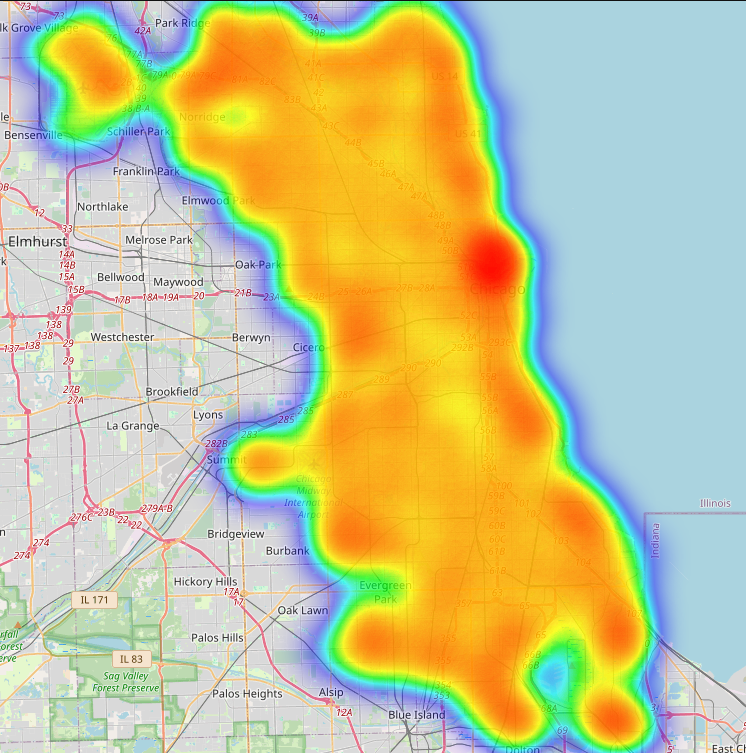
\includegraphics[height=8cm]{karte_Chicago_Heatmap}
\end{center}
        
    Aus der Verteilung der Verbrechen in Chicago kann man den Schluss
ziehen, das es in dichter besiedelten Gebieten mehr Verbrechen gibt. Um
dies zu bestätigen, können wir mit der Folium Library auch einen
Vergleich der Heatmap mit einer leeren Satellitenkarte herstellen.

\subsubsection{Vergleich mit
Satellitenbildern}\label{vergleich-mit-satellitenbildern}

Dafür erstellen wir zuerst ein neues Folium DualMap Kartenobjekt
``vergleich'':

    \begin{tcolorbox}[breakable, size=fbox, boxrule=1pt, pad at break*=1mm,colback=cellbackground, colframe=cellborder]
\prompt{In}{incolor}{10}{\boxspacing}
\begin{Verbatim}[commandchars=\\\{\}]
\PY{n}{vergleich} \PY{o}{=} \PY{n}{fl}\PY{o}{.}\PY{n}{plugins}\PY{o}{.}\PY{n}{DualMap}\PY{p}{(}\PY{n}{location}\PY{o}{=}\PY{p}{(}\PY{l+m+mf}{41.849429}\PY{p}{,} \PY{o}{\PYZhy{}}\PY{l+m+mf}{87.597334}\PY{p}{)}\PY{p}{,} \PY{n}{tiles}\PY{o}{=}\PY{k+kc}{None}\PY{p}{,} \PY{n}{zoom\PYZus{}start}\PY{o}{=}\PY{l+m+mi}{11}\PY{p}{,} \PY{n}{control\PYZus{}scale}\PY{o}{=}\PY{k+kc}{True}\PY{p}{,}\PY{p}{)}
\end{Verbatim}
\end{tcolorbox}

    Daraufhin erstellen wir die zwei untergeordneten Kartenobjekte m1 und
m2, die zum Dualmap Kartenobjekt ``vergleich'' gehören. Als Kartenquelle
fügen wir für beide Karten die API der Satellitenkarte ``Esri World
Imagery'' ein, die frei verfügbar ist:

https://www.arcgis.com/home/item.html?id=10df2279f9684e4a9f6a7f08febac2a9

    \begin{tcolorbox}[breakable, size=fbox, boxrule=1pt, pad at break*=1mm,colback=cellbackground, colframe=cellborder]
\prompt{In}{incolor}{11}{\boxspacing}
\begin{Verbatim}[commandchars=\\\{\}]
\PY{n}{fl}\PY{o}{.}\PY{n}{TileLayer}\PY{p}{(}
    \PY{n}{tiles}\PY{o}{=}\PY{l+s+s1}{\PYZsq{}}\PY{l+s+s1}{https://server.arcgisonline.com/ArcGIS/rest/services/World\PYZus{}Imagery/MapServer/tile/}\PY{l+s+si}{\PYZob{}z\PYZcb{}}\PY{l+s+s1}{/}\PY{l+s+si}{\PYZob{}y\PYZcb{}}\PY{l+s+s1}{/}\PY{l+s+si}{\PYZob{}x\PYZcb{}}\PY{l+s+s1}{\PYZsq{}}\PY{p}{,}
    \PY{n}{attr}\PY{o}{=}\PY{l+s+s1}{\PYZsq{}}\PY{l+s+s1}{Esri}\PY{l+s+s1}{\PYZsq{}}\PY{p}{,}
    \PY{n}{name}\PY{o}{=}\PY{l+s+s1}{\PYZsq{}}\PY{l+s+s1}{Esri World Imagery}\PY{l+s+s1}{\PYZsq{}}\PY{p}{,}
\PY{p}{)}\PY{o}{.}\PY{n}{add\PYZus{}to}\PY{p}{(}\PY{n}{vergleich}\PY{o}{.}\PY{n}{m1}\PY{p}{)}\PY{p}{;}
\PY{n}{fl}\PY{o}{.}\PY{n}{TileLayer}\PY{p}{(}
    \PY{n}{tiles}\PY{o}{=}\PY{l+s+s1}{\PYZsq{}}\PY{l+s+s1}{https://server.arcgisonline.com/ArcGIS/rest/services/World\PYZus{}Imagery/MapServer/tile/}\PY{l+s+si}{\PYZob{}z\PYZcb{}}\PY{l+s+s1}{/}\PY{l+s+si}{\PYZob{}y\PYZcb{}}\PY{l+s+s1}{/}\PY{l+s+si}{\PYZob{}x\PYZcb{}}\PY{l+s+s1}{\PYZsq{}}\PY{p}{,}
    \PY{n}{attr}\PY{o}{=}\PY{l+s+s1}{\PYZsq{}}\PY{l+s+s1}{Esri}\PY{l+s+s1}{\PYZsq{}}\PY{p}{,}
    \PY{n}{name}\PY{o}{=}\PY{l+s+s1}{\PYZsq{}}\PY{l+s+s1}{Esri World Imagery}\PY{l+s+s1}{\PYZsq{}}\PY{p}{,}
\PY{p}{)}\PY{o}{.}\PY{n}{add\PYZus{}to}\PY{p}{(}\PY{n}{vergleich}\PY{o}{.}\PY{n}{m2}\PY{p}{)}\PY{p}{;}
\end{Verbatim}
\end{tcolorbox}

    Nun fügen wir wie oben die im Array ``lats\_longs'' gespeicherten
Koordinaten der Verbrechen als Heatmap zur ``m1'' Karte hinzu und zeigen
die neue ``vergleich'' Karte danach an:

    \begin{tcolorbox}[breakable, size=fbox, boxrule=1pt, pad at break*=1mm,colback=cellbackground, colframe=cellborder]
\prompt{In}{incolor}{12}{\boxspacing}
\begin{Verbatim}[commandchars=\\\{\}]
\PY{n}{HeatMap}\PY{p}{(}\PY{n}{lat\PYZus{}long}\PY{p}{,} \PY{n}{radius}\PY{o}{=}\PY{p}{(}\PY{l+m+mi}{30}\PY{p}{)}\PY{p}{,} \PY{n}{blur}\PY{o}{=}\PY{p}{(}\PY{l+m+mi}{28}\PY{p}{)}\PY{p}{)}\PY{o}{.}\PY{n}{add\PYZus{}to}\PY{p}{(}\PY{n}{vergleich}\PY{o}{.}\PY{n}{m1}\PY{p}{)}
\PY{c+c1}{\PYZsh{}Steuerungsobjekte hinzufügen}
\PY{n}{fl}\PY{o}{.}\PY{n}{LayerControl}\PY{p}{(}\PY{n}{collapsed}\PY{o}{=}\PY{k+kc}{True}\PY{p}{,} \PY{n}{show}\PY{o}{=}\PY{k+kc}{False}\PY{p}{)}\PY{o}{.}\PY{n}{add\PYZus{}to}\PY{p}{(}\PY{n}{vergleich}\PY{p}{)}

\PY{c+c1}{\PYZsh{}Karte ausgeben und speichern}
\PY{n}{vergleich}\PY{o}{.}\PY{n}{save}\PY{p}{(}\PY{l+s+s1}{\PYZsq{}}\PY{l+s+s1}{Karten/Chicago\PYZus{}Vergleich\PYZus{}Heatmap\PYZus{}Satellit.html}\PY{l+s+s1}{\PYZsq{}}\PY{p}{)}
\PY{n}{vergleich}
\end{Verbatim}
\end{tcolorbox}

            \begin{tcolorbox}[breakable, size=fbox, boxrule=.5pt, pad at break*=1mm, opacityfill=0]
\prompt{Out}{outcolor}{12}{\boxspacing}
\begin{Verbatim}[commandchars=\\\{\}]
<folium.plugins.dual\_map.DualMap at 0x26683e0bcd0>
\end{Verbatim}
\end{tcolorbox}

\begin{center}
  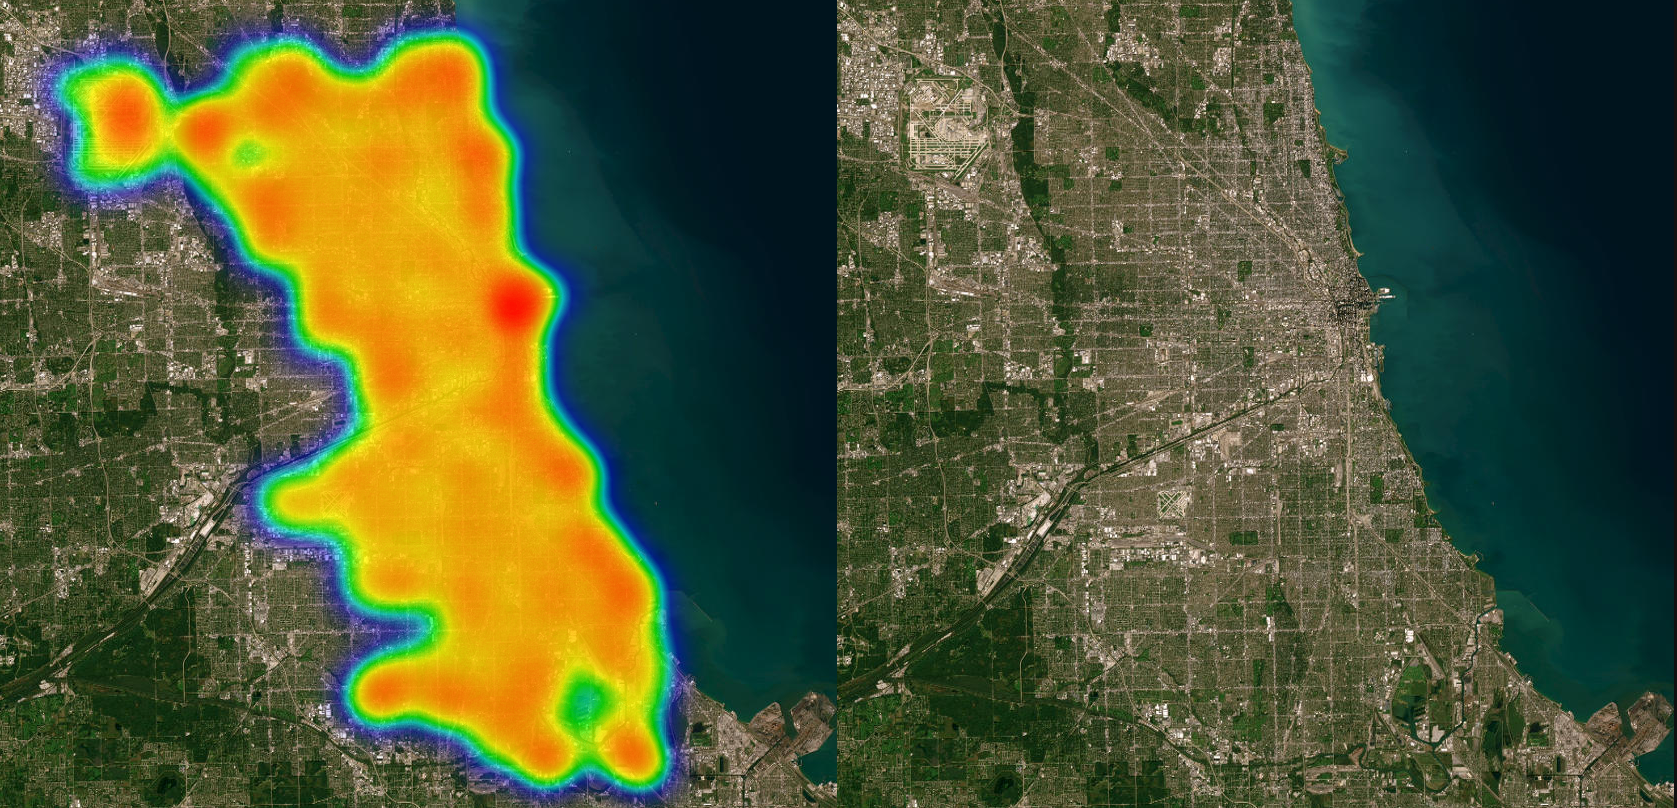
\includegraphics[height=8cm]{vergleich}
\end{center}
        
    Es ist erkennbar, dass an manchen Orten die Bebauungsdichte mit der
Verbrechenshäufigkeit korreliert. Besonders in Downtown Chicago ist das
der Fall. Auf dem Rest der Karte ist diese Korrelation aber meist nicht
aufzufinden. Deshalb kann man nicht generell sagen, dass eine hohe
Bebauungsdichte (und somit in der Regel auch eine hohe
Bevölkerungsdichte) immer zu einer erhöhten Verbrechenshäufigkeit führt.

    \subsubsection{Anwendung auf bestimmte
Reiseziele}\label{anwendung-auf-bestimmte-reiseziele}

Um nun konkretere Reiseempfehlungen treffen zu können, sollte man
interessante Reiseziele oder Hotels erst in dieser Karte aufsuchen, um
deren Sicherheit zu bestimmen. Als Beispiel fügen wir einige Hotels mit
deren Koordinaten in der Karte als Marker ein:

    \begin{tcolorbox}[breakable, size=fbox, boxrule=1pt, pad at break*=1mm,colback=cellbackground, colframe=cellborder]
\prompt{In}{incolor}{13}{\boxspacing}
\begin{Verbatim}[commandchars=\\\{\}]
\PY{c+c1}{\PYZsh{}Refernenzkopie der Karte auf ein neues Kartenobjekt, Zentrieren auf die Koordinaten von Hotel 2}
\PY{n}{marker\PYZus{}Chicago\PYZus{}Heatmap} \PY{o}{=} \PY{n}{karte\PYZus{}Chicago\PYZus{}Heatmap}
\PY{n}{marker\PYZus{}Chicago\PYZus{}Heatmap}\PY{o}{.}\PY{n}{zoom\PYZus{}start}\PY{o}{=} \PY{l+m+mi}{11}
\PY{n}{marker\PYZus{}Chicago\PYZus{}Heatmap}\PY{o}{.}\PY{n}{location}\PY{o}{=} \PY{p}{[}\PY{l+m+mf}{41.88612445681384}\PY{p}{,} \PY{o}{\PYZhy{}}\PY{l+m+mf}{87.63367468354781}\PY{p}{]}

\PY{c+c1}{\PYZsh{}Hotelmarker hinzufügen}
\PY{n}{fl}\PY{o}{.}\PY{n}{Marker}\PY{p}{(}
    \PY{n}{location}\PY{o}{=}\PY{p}{[}\PY{l+m+mf}{41.895194867728925}\PY{p}{,} \PY{o}{\PYZhy{}}\PY{l+m+mf}{87.61606169978471}\PY{p}{]}\PY{p}{,}
    \PY{n}{tooltip}\PY{o}{=}\PY{l+s+s2}{\PYZdq{}}\PY{l+s+s2}{W Chicago \PYZhy{} Lakeshore}\PY{l+s+s2}{\PYZdq{}}\PY{p}{,}
    \PY{n}{popup}\PY{o}{=}\PY{l+s+s2}{\PYZdq{}}\PY{l+s+s2}{https://maps.app.goo.gl/kRhLEB6UwdkJGLiJA}\PY{l+s+s2}{\PYZdq{}}\PY{p}{,}
    \PY{n}{icon}\PY{o}{=}\PY{n}{fl}\PY{o}{.}\PY{n}{Icon}\PY{p}{(}\PY{n}{color}\PY{o}{=}\PY{l+s+s2}{\PYZdq{}}\PY{l+s+s2}{red}\PY{l+s+s2}{\PYZdq{}}\PY{p}{,} \PY{n}{icon}\PY{o}{=}\PY{l+s+s2}{\PYZdq{}}\PY{l+s+s2}{1}\PY{l+s+s2}{\PYZdq{}}\PY{p}{,} \PY{n}{prefix}\PY{o}{=}\PY{l+s+s1}{\PYZsq{}}\PY{l+s+s1}{fa}\PY{l+s+s1}{\PYZsq{}}\PY{p}{,}\PY{p}{)}\PY{p}{,}\PY{p}{)}\PY{o}{.}\PY{n}{add\PYZus{}to}\PY{p}{(}\PY{n}{marker\PYZus{}Chicago\PYZus{}Heatmap}\PY{p}{)}\PY{p}{;}
\PY{n}{fl}\PY{o}{.}\PY{n}{Marker}\PY{p}{(}
    \PY{n}{location}\PY{o}{=}\PY{p}{[}\PY{l+m+mf}{41.88612445681384}\PY{p}{,} \PY{o}{\PYZhy{}}\PY{l+m+mf}{87.63367468354781}\PY{p}{]}\PY{p}{,}
    \PY{n}{tooltip}\PY{o}{=}\PY{l+s+s2}{\PYZdq{}}\PY{l+s+s2}{The Allegro Royal Sonesta Hotel Chicago Loop}\PY{l+s+s2}{\PYZdq{}}\PY{p}{,}
    \PY{n}{popup}\PY{o}{=}\PY{l+s+s2}{\PYZdq{}}\PY{l+s+s2}{https://maps.app.goo.gl/eNWMsavhf1eFtzj47}\PY{l+s+s2}{\PYZdq{}}\PY{p}{,}
    \PY{n}{icon}\PY{o}{=}\PY{n}{fl}\PY{o}{.}\PY{n}{Icon}\PY{p}{(}\PY{n}{color}\PY{o}{=}\PY{l+s+s2}{\PYZdq{}}\PY{l+s+s2}{red}\PY{l+s+s2}{\PYZdq{}}\PY{p}{,} \PY{n}{icon}\PY{o}{=}\PY{l+s+s2}{\PYZdq{}}\PY{l+s+s2}{2}\PY{l+s+s2}{\PYZdq{}}\PY{p}{,} \PY{n}{prefix}\PY{o}{=}\PY{l+s+s1}{\PYZsq{}}\PY{l+s+s1}{fa}\PY{l+s+s1}{\PYZsq{}}\PY{p}{,}\PY{p}{)}\PY{p}{,}\PY{p}{)}\PY{o}{.}\PY{n}{add\PYZus{}to}\PY{p}{(}\PY{n}{marker\PYZus{}Chicago\PYZus{}Heatmap}\PY{p}{)}\PY{p}{;}
\PY{n}{fl}\PY{o}{.}\PY{n}{Marker}\PY{p}{(}
    \PY{n}{location}\PY{o}{=}\PY{p}{[}\PY{l+m+mf}{41.8378989795599}\PY{p}{,} \PY{o}{\PYZhy{}}\PY{l+m+mf}{87.65697241489531}\PY{p}{]}\PY{p}{,}
    \PY{n}{tooltip}\PY{o}{=}\PY{l+s+s2}{\PYZdq{}}\PY{l+s+s2}{The Polo Inn Bed \PYZam{} Breakfast}\PY{l+s+s2}{\PYZdq{}}\PY{p}{,}
    \PY{n}{popup}\PY{o}{=}\PY{l+s+s2}{\PYZdq{}}\PY{l+s+s2}{https://maps.app.goo.gl/U61Rx65AYDoEDjsu9}\PY{l+s+s2}{\PYZdq{}}\PY{p}{,}
    \PY{n}{icon}\PY{o}{=}\PY{n}{fl}\PY{o}{.}\PY{n}{Icon}\PY{p}{(}\PY{n}{color}\PY{o}{=}\PY{l+s+s2}{\PYZdq{}}\PY{l+s+s2}{red}\PY{l+s+s2}{\PYZdq{}}\PY{p}{,} \PY{n}{icon}\PY{o}{=}\PY{l+s+s2}{\PYZdq{}}\PY{l+s+s2}{3}\PY{l+s+s2}{\PYZdq{}}\PY{p}{,} \PY{n}{prefix}\PY{o}{=}\PY{l+s+s1}{\PYZsq{}}\PY{l+s+s1}{fa}\PY{l+s+s1}{\PYZsq{}}\PY{p}{,}\PY{p}{)}\PY{p}{,}\PY{p}{)}\PY{o}{.}\PY{n}{add\PYZus{}to}\PY{p}{(}\PY{n}{marker\PYZus{}Chicago\PYZus{}Heatmap}\PY{p}{)}\PY{p}{;}

\PY{c+c1}{\PYZsh{}Karte ausgeben und speichern}
\PY{n}{marker\PYZus{}Chicago\PYZus{}Heatmap}\PY{o}{.}\PY{n}{save}\PY{p}{(}\PY{l+s+s1}{\PYZsq{}}\PY{l+s+s1}{Karten/Chicago\PYZus{}Heatmap\PYZus{}Marker.html}\PY{l+s+s1}{\PYZsq{}}\PY{p}{)}
\PY{n}{marker\PYZus{}Chicago\PYZus{}Heatmap}
\end{Verbatim}
\end{tcolorbox}

            \begin{tcolorbox}[breakable, size=fbox, boxrule=.5pt, pad at break*=1mm, opacityfill=0]
\prompt{Out}{outcolor}{13}{\boxspacing}
\begin{Verbatim}[commandchars=\\\{\}]
<folium.folium.Map at 0x266264b7310>
\end{Verbatim}
\end{tcolorbox}
        
    Durch einen Klick mit dem Mauszeiger kann auch direkt auf der Karte der
Name des Hotels und der entsprechende Google Maps link eingesehen
werden. Da aber nicht jeder die Karte interaktiv zur Hand haben wird,
sind hier auch noch einmal die Informationen sowie die
Sicherheitseinschätzung des Gebiets dem Datensatz zufolge aufgelistet:

1: Das ``W Chicago - Lakeshore'' Hotel ist offensichtlich keine gute
Wahl, da der roten Umgebungsfarbe nach zu urteilen die Umgebung nicht
sehr sicher ist.\\
2: Das ``The Allegro Royal Sonesta Hotel Chicago Loop'' Hotel liegt in
einem sehr roten Bereich, deshalb ist dem Datensatz nachzuschließen auch
dieses Hotel und der umliegende Bereich zu meiden.\\
3: Das ``The Polo Inn Bed \& Breakfast'' Hotel dagegen ist im Vergleich
zum Rest von Chicago in einem sichereren Bereich, und ist deshalb dem
Datensatz zufolge zu empfehlen

\subsubsection{Anwendung auf andere
Hotels/Reiseziele}\label{anwendung-auf-andere-hotelsreiseziele}

\paragraph{Manuelle Verwendung der
Karte}\label{manuelle-verwendung-der-karte}

Um ein anderes Hotel einschätzen zu können, müssen folgende Schritte
befolgt werden:\\
1: Ein Hotel auf einem Kartedienst finden (z.B. Google Maps)\\
2: Das Hotel visuell auf der Heatmap aufsuchen und die Röte des Gebiets
im Vergleich zum Rest der Heatmap begutachten\\
3: Je nach Tiefe der Röte entscheiden, ob der Ort den
Sicherheitsanforderungen entspricht

\paragraph{Abfragen basierte Verwendung der
Karte}\label{abfragen-basierte-verwendung-der-karte}

Wie im Kapitel Deployment beschrieben, ist auch eine interaktive
Verwendung möglich.

    \subsection{Sichere Tageszeiten?}\label{sichere-tageszeiten}

    Hier stellen wir die jeweiligen Tageszeiten, zu denen Verbrechen
geschehen sind, als Histogramm dar. Wir müssen zuerst die Date Spalte
von Objects zu Datetimes konvertieren, um dann mit diesen einen Plot
erstellen zu können, indem wir aus der Datetime direkt die Stunde
rausziehen.

    \begin{tcolorbox}[breakable, size=fbox, boxrule=1pt, pad at break*=1mm,colback=cellbackground, colframe=cellborder]
\prompt{In}{incolor}{14}{\boxspacing}
\begin{Verbatim}[commandchars=\\\{\}]
\PY{c+c1}{\PYZsh{}Umformatierung der Daten zu Datetimes}
\PY{n}{data\PYZus{}cleaned}\PY{p}{[}\PY{l+s+s1}{\PYZsq{}}\PY{l+s+s1}{Date}\PY{l+s+s1}{\PYZsq{}}\PY{p}{]} \PY{o}{=} \PY{n}{pd}\PY{o}{.}\PY{n}{to\PYZus{}datetime}\PY{p}{(}\PY{n}{data\PYZus{}cleaned}\PY{p}{[}\PY{l+s+s1}{\PYZsq{}}\PY{l+s+s1}{Date}\PY{l+s+s1}{\PYZsq{}}\PY{p}{]}\PY{p}{,} \PY{n+nb}{format}\PY{o}{=}\PY{l+s+s1}{\PYZsq{}}\PY{l+s+s1}{\PYZpc{}}\PY{l+s+s1}{m/}\PY{l+s+si}{\PYZpc{}d}\PY{l+s+s1}{/}\PY{l+s+s1}{\PYZpc{}}\PY{l+s+s1}{Y }\PY{l+s+s1}{\PYZpc{}}\PY{l+s+s1}{I:}\PY{l+s+s1}{\PYZpc{}}\PY{l+s+s1}{M:}\PY{l+s+s1}{\PYZpc{}}\PY{l+s+s1}{S }\PY{l+s+s1}{\PYZpc{}}\PY{l+s+s1}{p}\PY{l+s+s1}{\PYZsq{}}\PY{p}{)}
\PY{n}{day\PYZus{}of\PYZus{}month\PYZus{}chicago\PYZus{}crime\PYZus{}data} \PY{o}{=} \PY{n}{data\PYZus{}cleaned}\PY{p}{[}\PY{l+s+s1}{\PYZsq{}}\PY{l+s+s1}{Date}\PY{l+s+s1}{\PYZsq{}}\PY{p}{]}\PY{o}{.}\PY{n}{dt}\PY{o}{.}\PY{n}{hour}
\PY{n}{fig} \PY{o}{=} \PY{n}{sns}\PY{o}{.}\PY{n}{histplot}\PY{p}{(}\PY{n}{day\PYZus{}of\PYZus{}month\PYZus{}chicago\PYZus{}crime\PYZus{}data}\PY{p}{,} \PY{n}{kde}\PY{o}{=}\PY{k+kc}{False}\PY{p}{,} \PY{n}{bins}\PY{o}{=}\PY{l+m+mi}{24}\PY{p}{)}
\PY{n}{fig}\PY{o}{.}\PY{n}{set}\PY{p}{(}\PY{n}{xlabel}\PY{o}{=}\PY{l+s+s1}{\PYZsq{}}\PY{l+s+s1}{Hour}\PY{l+s+s1}{\PYZsq{}}\PY{p}{,} \PY{n}{ylabel}\PY{o}{=}\PY{l+s+s1}{\PYZsq{}}\PY{l+s+s1}{Amount of commited Crimes}\PY{l+s+s1}{\PYZsq{}}\PY{p}{)}\PY{p}{;}
\end{Verbatim}
\end{tcolorbox}

    \begin{center}
    \adjustimage{max size={0.9\linewidth}{0.9\paperheight}}{output_37_0.png}
    \end{center}
    { \hspace*{\fill} \\}
    
    Im Histogramm können wir nun die Tageszeiten der begangenen Verbrechen
sehen. Man sieht deutlich, dass nachts (5 Uhr) am wenigsten Verbrechen
geschehen, und diese fast stetig bis 18 Uhr zunehmen, und diese Anzahl
sich wieder bis 5 Uhr verringert. Ausnahme davon sind 0 und 12 Uhr,
unsere Vermutung hier ist, dass Verbrechen, bei denen nur eine ungefähre
Uhrzeit zur Verfügung stand, entweder auf 0 oder auf 12 Uhr
ab/aufgerundet wurden.

Auf ersten Blick würde man also denken, dass die sicherste Tageszeit für
einen Trip die Nacht wäre, aber da nachts normalerweise weniger Menschen
aktiv sind, ist diese Statistik etwas trügerisch. Unser Fazit hier ist,
dass wir aus diesem Histogramm leider keine erkenntliche Einsicht über
eine empfehlenswerte Tageszeit zum Rausgehen gewinnen können.

    \subsection{Sichere Jahreszeiten?}\label{sichere-jahreszeiten}

    Wir fangen an, indem wir eine Methode definieren, die uns die Jahreszeit
je nach Monat angibt. Danach erstellen wir eine neue Spalte, die uns die
Jahreszeit des jeweiligen Verbrechens zurückgibt. Wir erstellen
daraufhin ein Balkendiagramm, dass uns eine visuelle Übersicht über die
jeweilige Jahreszeit gibt.

    \begin{tcolorbox}[breakable, size=fbox, boxrule=1pt, pad at break*=1mm,colback=cellbackground, colframe=cellborder]
\prompt{In}{incolor}{15}{\boxspacing}
\begin{Verbatim}[commandchars=\\\{\}]
\PY{k}{def} \PY{n+nf}{get\PYZus{}season}\PY{p}{(}\PY{n}{date}\PY{p}{)}\PY{p}{:}
    \PY{n}{month} \PY{o}{=} \PY{n}{date}\PY{o}{.}\PY{n}{month}
    \PY{k}{if} \PY{l+m+mi}{3} \PY{o}{\PYZlt{}}\PY{o}{=} \PY{n}{month} \PY{o}{\PYZlt{}}\PY{o}{=} \PY{l+m+mi}{5}\PY{p}{:}
        \PY{k}{return} \PY{l+s+s2}{\PYZdq{}}\PY{l+s+s2}{Frühling}\PY{l+s+s2}{\PYZdq{}}
    \PY{k}{elif} \PY{l+m+mi}{6} \PY{o}{\PYZlt{}}\PY{o}{=} \PY{n}{month} \PY{o}{\PYZlt{}}\PY{o}{=} \PY{l+m+mi}{8}\PY{p}{:}
        \PY{k}{return} \PY{l+s+s2}{\PYZdq{}}\PY{l+s+s2}{Sommer}\PY{l+s+s2}{\PYZdq{}}
    \PY{k}{elif} \PY{l+m+mi}{9} \PY{o}{\PYZlt{}}\PY{o}{=} \PY{n}{month} \PY{o}{\PYZlt{}}\PY{o}{=} \PY{l+m+mi}{11}\PY{p}{:}
        \PY{k}{return} \PY{l+s+s2}{\PYZdq{}}\PY{l+s+s2}{Herbst}\PY{l+s+s2}{\PYZdq{}}
    \PY{k}{else}\PY{p}{:}
        \PY{k}{return} \PY{l+s+s2}{\PYZdq{}}\PY{l+s+s2}{Winter}\PY{l+s+s2}{\PYZdq{}}

\PY{n}{data\PYZus{}cleaned}\PY{p}{[}\PY{l+s+s1}{\PYZsq{}}\PY{l+s+s1}{Jahreszeit}\PY{l+s+s1}{\PYZsq{}}\PY{p}{]} \PY{o}{=} \PY{n}{data\PYZus{}cleaned}\PY{p}{[}\PY{l+s+s1}{\PYZsq{}}\PY{l+s+s1}{Date}\PY{l+s+s1}{\PYZsq{}}\PY{p}{]}\PY{o}{.}\PY{n}{apply}\PY{p}{(}\PY{n}{get\PYZus{}season}\PY{p}{)}

\PY{n}{chicago\PYZus{}crime\PYZus{}data\PYZus{}grouped} \PY{o}{=} \PY{n}{data\PYZus{}cleaned}\PY{o}{.}\PY{n}{groupby}\PY{p}{(}\PY{l+s+s1}{\PYZsq{}}\PY{l+s+s1}{Jahreszeit}\PY{l+s+s1}{\PYZsq{}}\PY{p}{)}\PY{p}{[}\PY{l+s+s1}{\PYZsq{}}\PY{l+s+s1}{Case Number}\PY{l+s+s1}{\PYZsq{}}\PY{p}{]}\PY{o}{.}\PY{n}{size}\PY{p}{(}\PY{p}{)}

\PY{n}{plt}\PY{o}{.}\PY{n}{bar}\PY{p}{(}\PY{n}{chicago\PYZus{}crime\PYZus{}data\PYZus{}grouped}\PY{o}{.}\PY{n}{index}\PY{p}{,} \PY{n}{chicago\PYZus{}crime\PYZus{}data\PYZus{}grouped}\PY{o}{.}\PY{n}{values}\PY{p}{,} \PY{n}{color}\PY{o}{=}\PY{p}{[}\PY{l+s+s1}{\PYZsq{}}\PY{l+s+s1}{green}\PY{l+s+s1}{\PYZsq{}}\PY{p}{,} \PY{l+s+s1}{\PYZsq{}}\PY{l+s+s1}{orange}\PY{l+s+s1}{\PYZsq{}}\PY{p}{,} \PY{l+s+s1}{\PYZsq{}}\PY{l+s+s1}{red}\PY{l+s+s1}{\PYZsq{}}\PY{p}{,} \PY{l+s+s1}{\PYZsq{}}\PY{l+s+s1}{blue}\PY{l+s+s1}{\PYZsq{}}\PY{p}{]}\PY{p}{)}
\PY{n}{plt}\PY{o}{.}\PY{n}{title}\PY{p}{(}\PY{l+s+s1}{\PYZsq{}}\PY{l+s+s1}{Balkendiagramm nach Jahreszeiten}\PY{l+s+s1}{\PYZsq{}}\PY{p}{)}
\PY{n}{plt}\PY{o}{.}\PY{n}{xlabel}\PY{p}{(}\PY{l+s+s1}{\PYZsq{}}\PY{l+s+s1}{Jahreszeit}\PY{l+s+s1}{\PYZsq{}}\PY{p}{)}
\PY{n}{plt}\PY{o}{.}\PY{n}{ylabel}\PY{p}{(}\PY{l+s+s1}{\PYZsq{}}\PY{l+s+s1}{Summe der Werte}\PY{l+s+s1}{\PYZsq{}}\PY{p}{)}
\PY{n}{plt}\PY{o}{.}\PY{n}{show}\PY{p}{(}\PY{p}{)}
\end{Verbatim}
\end{tcolorbox}

    \begin{center}
    \adjustimage{max size={0.9\linewidth}{0.9\paperheight}}{output_41_0.png}
    \end{center}
    { \hspace*{\fill} \\}
    
    Man kann deutlich sehen, dass die Anzahl der Verbrechen im Vergleich zu
den Anderen Jahreszeiten im Winter stark sinkt, während im Sommer mehr
Verbrechen geschehen. Für einen Trip nach Chicago würde sich also
definitiv der Winter anbieten!

    \subsection{Klassifizierung der
Verbrechen}\label{klassifizierung-der-verbrechen}

\subsubsection{Klassifizierung}\label{klassifizierung}

    In unserem Datensatz sowie im echten Leben gibt es viele verschiedene
Verbrechenskategorien. Diese variieren von vergleichsweise harmlosen
Gesetzesverstößen wie Taschendiebstahl bis hin zu schweren Verbrechen
wie Mord. Nicht alle Verbrechen betreffen uns aber als Urlauber in
Chicago. `LIQUOR LAW VIOLATION', d.h. ein Spirituosen Gesetzes Verstoß
betrifft und als Urlauber nicht, obwohl es durchaus für die Stadt ein
größeres Problem darstellen könnte. Deshalb teilen wir die vielen
verschiedenen Verbrechensarten in die zwei Kategorien
schwerwiegend\_Urlaub und belanglos\_Urlaub ein. Besonders
schwerwiegende Verbrechen, wie zum Beispiel solche, die schwere Sach-,
Personen- oder psychische Schäden verursachen werden und von welchen wir
als Urlauber ebenfalls potenziell betroffen sein könnten, werden als
schwerwiegend eingestuft, Verbrechen die eher geringfügige Schäden
verursachen werden hingegen als weniger schwerwiegend eingestuft.

Dazu rufen wir zunächst alle einzigartigen Verbrechensarten in der
Kategorie `Primary Type' auf und geben die daraus resultierende Liste
mit print() aus:

    \begin{tcolorbox}[breakable, size=fbox, boxrule=1pt, pad at break*=1mm,colback=cellbackground, colframe=cellborder]
\prompt{In}{incolor}{16}{\boxspacing}
\begin{Verbatim}[commandchars=\\\{\}]
\PY{n}{unique\PYZus{}types} \PY{o}{=} \PY{n}{data\PYZus{}cleaned}\PY{p}{[}\PY{l+s+s1}{\PYZsq{}}\PY{l+s+s1}{Primary Type}\PY{l+s+s1}{\PYZsq{}}\PY{p}{]}\PY{o}{.}\PY{n}{unique}\PY{p}{(}\PY{p}{)}
\PY{n+nb}{print}\PY{p}{(}\PY{n}{unique\PYZus{}types}\PY{p}{)}
\end{Verbatim}
\end{tcolorbox}

    \begin{Verbatim}[commandchars=\\\{\}]
['CRIMINAL DAMAGE' 'DECEPTIVE PRACTICE' 'CRIMINAL SEXUAL ASSAULT' 'THEFT'
 'ROBBERY' 'SEX OFFENSE' 'WEAPONS VIOLATION' 'STALKING'
 'MOTOR VEHICLE THEFT' 'CRIMINAL TRESPASS' 'BATTERY' 'OTHER OFFENSE'
 'HOMICIDE' 'PROSTITUTION' 'BURGLARY' 'ASSAULT' 'NARCOTICS' 'KIDNAPPING'
 'ARSON' 'CONCEALED CARRY LICENSE VIOLATION'
 'INTERFERENCE WITH PUBLIC OFFICER' 'PUBLIC PEACE VIOLATION'
 'OFFENSE INVOLVING CHILDREN' 'LIQUOR LAW VIOLATION' 'INTIMIDATION'
 'GAMBLING' 'OBSCENITY' 'HUMAN TRAFFICKING' 'CRIM SEXUAL ASSAULT'
 'OTHER NARCOTIC VIOLATION' 'PUBLIC INDECENCY' 'RITUALISM' 'NON-CRIMINAL'
 'NON-CRIMINAL (SUBJECT SPECIFIED)' 'NON - CRIMINAL']
    \end{Verbatim}

    Nach einiger Überlegung und Evaluation stufen wir nun die folgenden
Verbrechen als schwerwiegend für Urlauber ein: `THEFT', `ASSAULT',
`WEAPONS VIOLATION',`SEX OFFENSE',`CRIM SEXUAL ASSAULT',`MOTOR VEHICLE
THEFT',`CRIMINAL TRESPASS',`ROBBERY',`PUBLIC PEACE VIOLATION',`CRIMINAL
SEXUAL ASSAULT',`HOMICIDE', `KIDNAPPING' und `HUMAN TRAFFICKING'. Diese
werden in der Liste schwerwiegend\_Urlaub als Zeichenkette gespeichert:

    \begin{tcolorbox}[breakable, size=fbox, boxrule=1pt, pad at break*=1mm,colback=cellbackground, colframe=cellborder]
\prompt{In}{incolor}{17}{\boxspacing}
\begin{Verbatim}[commandchars=\\\{\}]
\PY{n}{schwerwiegend\PYZus{}Urlaub} \PY{o}{=} \PY{p}{[}\PY{l+s+s1}{\PYZsq{}}\PY{l+s+s1}{THEFT}\PY{l+s+s1}{\PYZsq{}}\PY{p}{,} \PY{l+s+s1}{\PYZsq{}}\PY{l+s+s1}{ASSAULT}\PY{l+s+s1}{\PYZsq{}}\PY{p}{,} \PY{l+s+s1}{\PYZsq{}}\PY{l+s+s1}{WEAPONS VIOLATION}\PY{l+s+s1}{\PYZsq{}}\PY{p}{,}\PY{l+s+s1}{\PYZsq{}}\PY{l+s+s1}{SEX OFFENSE}\PY{l+s+s1}{\PYZsq{}}\PY{p}{,}\PY{l+s+s1}{\PYZsq{}}\PY{l+s+s1}{CRIM SEXUAL ASSAULT}\PY{l+s+s1}{\PYZsq{}}\PY{p}{,}\PY{l+s+s1}{\PYZsq{}}\PY{l+s+s1}{MOTOR VEHICLE THEFT}\PY{l+s+s1}{\PYZsq{}}\PY{p}{,}\PY{l+s+s1}{\PYZsq{}}\PY{l+s+s1}{CRIMINAL TRESPASS}\PY{l+s+s1}{\PYZsq{}}\PY{p}{,}\PY{l+s+s1}{\PYZsq{}}\PY{l+s+s1}{ROBBERY}\PY{l+s+s1}{\PYZsq{}}\PY{p}{,}\PY{l+s+s1}{\PYZsq{}}\PY{l+s+s1}{PUBLIC PEACE VIOLATION}\PY{l+s+s1}{\PYZsq{}}\PY{p}{,}\PY{l+s+s1}{\PYZsq{}}\PY{l+s+s1}{CRIMINAL SEXUAL ASSAULT}\PY{l+s+s1}{\PYZsq{}}\PY{p}{,}\PY{l+s+s1}{\PYZsq{}}\PY{l+s+s1}{HOMICIDE}\PY{l+s+s1}{\PYZsq{}}\PY{p}{,} \PY{l+s+s1}{\PYZsq{}}\PY{l+s+s1}{KIDNAPPING}\PY{l+s+s1}{\PYZsq{}}\PY{p}{,}\PY{l+s+s1}{\PYZsq{}}\PY{l+s+s1}{HUMAN TRAFFICKING}\PY{l+s+s1}{\PYZsq{}}\PY{p}{]}
\end{Verbatim}
\end{tcolorbox}

    Jetzt werden die Verbrechen im gesamten Datensatz bewertet und als
``Schwerwiegend'' oder ``Nicht Schwerwiegend'' entsprechend eingestuft.

Dazu erstellen wir die Methode ``klassifizieren''. Diese nimmt als
Parameter einen `crime\_type' String. Wenn dieser Parameter in der Liste
schwerwiegende\_verbrechen enthalten ist, gibt die Methode
`Schwerwiegend' aus, wenn nicht wird `Nicht Schwerwiegend' ausgegeben:

    \begin{tcolorbox}[breakable, size=fbox, boxrule=1pt, pad at break*=1mm,colback=cellbackground, colframe=cellborder]
\prompt{In}{incolor}{18}{\boxspacing}
\begin{Verbatim}[commandchars=\\\{\}]
\PY{k}{def} \PY{n+nf}{klassifizieren}\PY{p}{(}\PY{n}{crime\PYZus{}type}\PY{p}{)}\PY{p}{:}
    \PY{k}{if} \PY{n}{crime\PYZus{}type} \PY{o+ow}{in} \PY{n}{schwerwiegend\PYZus{}Urlaub}\PY{p}{:}
        \PY{k}{return} \PY{l+s+s1}{\PYZsq{}}\PY{l+s+s1}{Schwerwiegend}\PY{l+s+s1}{\PYZsq{}}
    \PY{k}{else}\PY{p}{:}
        \PY{k}{return} \PY{l+s+s1}{\PYZsq{}}\PY{l+s+s1}{Nicht Schwerwiegend}\PY{l+s+s1}{\PYZsq{}}


\PY{n}{data\PYZus{}cleaned}\PY{p}{[}\PY{l+s+s1}{\PYZsq{}}\PY{l+s+s1}{Schwere Klassifizierung}\PY{l+s+s1}{\PYZsq{}}\PY{p}{]} \PY{o}{=} \PY{n}{data\PYZus{}cleaned}\PY{p}{[}\PY{l+s+s1}{\PYZsq{}}\PY{l+s+s1}{Primary Type}\PY{l+s+s1}{\PYZsq{}}\PY{p}{]}\PY{o}{.}\PY{n}{apply}\PY{p}{(}\PY{n}{klassifizieren}\PY{p}{)}
\end{Verbatim}
\end{tcolorbox}

    \subsubsection{Gruppierung nach Jahren}\label{gruppierung-nach-jahren}

    Um die Analyse durchführen zu können, werden jetzt die Daten nach Jahren
gruppiert, und die Anzahl schwerwiegender und nicht schwerwiegender
Verbrechen für jedes Jahr summiert.

    \begin{tcolorbox}[breakable, size=fbox, boxrule=1pt, pad at break*=1mm,colback=cellbackground, colframe=cellborder]
\prompt{In}{incolor}{19}{\boxspacing}
\begin{Verbatim}[commandchars=\\\{\}]
\PY{n}{gruppe} \PY{o}{=} \PY{n}{data\PYZus{}cleaned}\PY{o}{.}\PY{n}{groupby}\PY{p}{(}\PY{p}{[}\PY{l+s+s1}{\PYZsq{}}\PY{l+s+s1}{Year}\PY{l+s+s1}{\PYZsq{}}\PY{p}{,} \PY{l+s+s1}{\PYZsq{}}\PY{l+s+s1}{Schwere Klassifizierung}\PY{l+s+s1}{\PYZsq{}}\PY{p}{]}\PY{p}{)}\PY{o}{.}\PY{n}{size}\PY{p}{(}\PY{p}{)}\PY{o}{.}\PY{n}{unstack}\PY{p}{(}\PY{p}{)}
\PY{n}{gruppe} \PY{o}{=} \PY{n}{gruppe}\PY{o}{.}\PY{n}{fillna}\PY{p}{(}\PY{l+m+mi}{0}\PY{p}{)}
\end{Verbatim}
\end{tcolorbox}

    Diese Daten werden jetzt zur Veranschaulichung in einem Diagramm
präsentiert:

    \begin{tcolorbox}[breakable, size=fbox, boxrule=1pt, pad at break*=1mm,colback=cellbackground, colframe=cellborder]
\prompt{In}{incolor}{20}{\boxspacing}
\begin{Verbatim}[commandchars=\\\{\}]
\PY{n}{gruppe}\PY{p}{[}\PY{l+s+s1}{\PYZsq{}}\PY{l+s+s1}{Schwerwiegend}\PY{l+s+s1}{\PYZsq{}}\PY{p}{]}\PY{o}{.}\PY{n}{plot}\PY{p}{(}\PY{n}{kind}\PY{o}{=}\PY{l+s+s1}{\PYZsq{}}\PY{l+s+s1}{line}\PY{l+s+s1}{\PYZsq{}}\PY{p}{,} \PY{n}{color}\PY{o}{=}\PY{l+s+s1}{\PYZsq{}}\PY{l+s+s1}{red}\PY{l+s+s1}{\PYZsq{}}\PY{p}{,} \PY{n}{marker}\PY{o}{=}\PY{l+s+s1}{\PYZsq{}}\PY{l+s+s1}{o}\PY{l+s+s1}{\PYZsq{}}\PY{p}{,} \PY{n}{label}\PY{o}{=}\PY{l+s+s1}{\PYZsq{}}\PY{l+s+s1}{Schwerwiegend}\PY{l+s+s1}{\PYZsq{}}\PY{p}{)}
\PY{n}{gruppe}\PY{p}{[}\PY{l+s+s1}{\PYZsq{}}\PY{l+s+s1}{Nicht Schwerwiegend}\PY{l+s+s1}{\PYZsq{}}\PY{p}{]}\PY{o}{.}\PY{n}{plot}\PY{p}{(}\PY{n}{kind}\PY{o}{=}\PY{l+s+s1}{\PYZsq{}}\PY{l+s+s1}{line}\PY{l+s+s1}{\PYZsq{}}\PY{p}{,} \PY{n}{color}\PY{o}{=}\PY{l+s+s1}{\PYZsq{}}\PY{l+s+s1}{gray}\PY{l+s+s1}{\PYZsq{}}\PY{p}{,} \PY{n}{marker}\PY{o}{=}\PY{l+s+s1}{\PYZsq{}}\PY{l+s+s1}{o}\PY{l+s+s1}{\PYZsq{}}\PY{p}{,} \PY{n}{label}\PY{o}{=}\PY{l+s+s1}{\PYZsq{}}\PY{l+s+s1}{Nicht Schwerwiegend}\PY{l+s+s1}{\PYZsq{}}\PY{p}{)}
\PY{n}{plt}\PY{o}{.}\PY{n}{title}\PY{p}{(}\PY{l+s+s1}{\PYZsq{}}\PY{l+s+s1}{Anzahl der schwerwiegenden und nicht\PYZhy{}schwerwiegenden Verbrechen pro Jahr}\PY{l+s+s1}{\PYZsq{}}\PY{p}{)}
\PY{n}{plt}\PY{o}{.}\PY{n}{grid}\PY{p}{(}\PY{n}{axis}\PY{o}{=}\PY{l+s+s1}{\PYZsq{}}\PY{l+s+s1}{x}\PY{l+s+s1}{\PYZsq{}}\PY{p}{,} \PY{n}{color}\PY{o}{=}\PY{l+s+s1}{\PYZsq{}}\PY{l+s+s1}{0.5}\PY{l+s+s1}{\PYZsq{}}\PY{p}{)}
\PY{n}{plt}\PY{o}{.}\PY{n}{xlabel}\PY{p}{(}\PY{l+s+s1}{\PYZsq{}}\PY{l+s+s1}{Jahr}\PY{l+s+s1}{\PYZsq{}}\PY{p}{)}
\PY{n}{plt}\PY{o}{.}\PY{n}{ylabel}\PY{p}{(}\PY{l+s+s1}{\PYZsq{}}\PY{l+s+s1}{Anzahl Verbrechen}\PY{l+s+s1}{\PYZsq{}}\PY{p}{)}
\PY{n}{plt}\PY{o}{.}\PY{n}{legend}\PY{p}{(}\PY{n}{title}\PY{o}{=}\PY{l+s+s1}{\PYZsq{}}\PY{l+s+s1}{Schwere Klassifizierung}\PY{l+s+s1}{\PYZsq{}}\PY{p}{)}
\PY{n}{plt}\PY{o}{.}\PY{n}{show}\PY{p}{(}\PY{p}{)}
\end{Verbatim}
\end{tcolorbox}

    \begin{center}
    \adjustimage{max size={0.9\linewidth}{0.9\paperheight}}{output_54_0.png}
    \end{center}
    { \hspace*{\fill} \\}
    
    Es ist zu erkennen, dass die Gesamtzahl an Verbrechen sich stark
reduziert hat. Aber es ist nicht wegzulassen, dass im Jahr 2022 die
Anzahl an für Urlauber relevante Verbrechen stark gewachsen ist.
Außerdem sind 2016 zum ersten Mal mehr Schwerwiegende als nicht
Schwerwiegende Verbrechen passiert.

Diesen Ergebnis wird nochmal tiefer untersucht, um zu sehen welche
konkrete verbrechen am meisten zugenommen haben.

    \begin{tcolorbox}[breakable, size=fbox, boxrule=1pt, pad at break*=1mm,colback=cellbackground, colframe=cellborder]
\prompt{In}{incolor}{21}{\boxspacing}
\begin{Verbatim}[commandchars=\\\{\}]
\PY{n}{schwere\PYZus{}verbrechen\PYZus{}2021} \PY{o}{=} \PY{n}{data\PYZus{}cleaned}\PY{p}{[}
    \PY{p}{(}\PY{n}{data\PYZus{}cleaned}\PY{p}{[}\PY{l+s+s1}{\PYZsq{}}\PY{l+s+s1}{Schwere Klassifizierung}\PY{l+s+s1}{\PYZsq{}}\PY{p}{]} \PY{o}{==} \PY{l+s+s1}{\PYZsq{}}\PY{l+s+s1}{Schwerwiegend}\PY{l+s+s1}{\PYZsq{}}\PY{p}{)} \PY{o}{\PYZam{}}
    \PY{p}{(}\PY{n}{data\PYZus{}cleaned}\PY{p}{[}\PY{l+s+s1}{\PYZsq{}}\PY{l+s+s1}{Year}\PY{l+s+s1}{\PYZsq{}}\PY{p}{]} \PY{o}{==} \PY{l+m+mi}{2021}\PY{p}{)}
\PY{p}{]}
\PY{n}{schwere\PYZus{}verbrechen\PYZus{}2022} \PY{o}{=} \PY{n}{data\PYZus{}cleaned}\PY{p}{[}
    \PY{p}{(}\PY{n}{data\PYZus{}cleaned}\PY{p}{[}\PY{l+s+s1}{\PYZsq{}}\PY{l+s+s1}{Schwere Klassifizierung}\PY{l+s+s1}{\PYZsq{}}\PY{p}{]} \PY{o}{==} \PY{l+s+s1}{\PYZsq{}}\PY{l+s+s1}{Schwerwiegend}\PY{l+s+s1}{\PYZsq{}}\PY{p}{)} \PY{o}{\PYZam{}}
    \PY{p}{(}\PY{n}{data\PYZus{}cleaned}\PY{p}{[}\PY{l+s+s1}{\PYZsq{}}\PY{l+s+s1}{Year}\PY{l+s+s1}{\PYZsq{}}\PY{p}{]} \PY{o}{==} \PY{l+m+mi}{2022}\PY{p}{)}
\PY{p}{]}
\end{Verbatim}
\end{tcolorbox}

    Daraufhin werden davon die Schwerwiegenden Verbrechen gruppiert und
extrahiert. Die nicht Schwerwiegenden werden ignoriert.

    \begin{tcolorbox}[breakable, size=fbox, boxrule=1pt, pad at break*=1mm,colback=cellbackground, colframe=cellborder]
\prompt{In}{incolor}{22}{\boxspacing}
\begin{Verbatim}[commandchars=\\\{\}]
\PY{n}{schwere\PYZus{}verbrechen\PYZus{}2021\PYZus{}anzahl} \PY{o}{=} \PY{n}{schwere\PYZus{}verbrechen\PYZus{}2021}\PY{o}{.}\PY{n}{groupby}\PY{p}{(}\PY{l+s+s1}{\PYZsq{}}\PY{l+s+s1}{Primary Type}\PY{l+s+s1}{\PYZsq{}}\PY{p}{)}\PY{o}{.}\PY{n}{size}\PY{p}{(}\PY{p}{)}\PY{o}{.}\PY{n}{sort\PYZus{}values}\PY{p}{(}\PY{n}{ascending}\PY{o}{=}\PY{k+kc}{False}\PY{p}{)}
\PY{n}{schwere\PYZus{}verbrechen\PYZus{}2022\PYZus{}anzahl} \PY{o}{=} \PY{n}{schwere\PYZus{}verbrechen\PYZus{}2022}\PY{o}{.}\PY{n}{groupby}\PY{p}{(}\PY{l+s+s1}{\PYZsq{}}\PY{l+s+s1}{Primary Type}\PY{l+s+s1}{\PYZsq{}}\PY{p}{)}\PY{o}{.}\PY{n}{size}\PY{p}{(}\PY{p}{)}\PY{o}{.}\PY{n}{sort\PYZus{}values}\PY{p}{(}\PY{n}{ascending}\PY{o}{=}\PY{k+kc}{False}\PY{p}{)}
\end{Verbatim}
\end{tcolorbox}

    Zuletzt wird für jede Art Schwerwiegender Verbrechen die Zunahme
berechnet und die Ergebnisse in einem Diagramm gezeigt.

    \begin{tcolorbox}[breakable, size=fbox, boxrule=1pt, pad at break*=1mm,colback=cellbackground, colframe=cellborder]
\prompt{In}{incolor}{23}{\boxspacing}
\begin{Verbatim}[commandchars=\\\{\}]
\PY{n}{zunahme\PYZus{}schwere\PYZus{}verbrechen\PYZus{}2022\PYZus{}vs\PYZus{}2021} \PY{o}{=} \PY{n}{schwere\PYZus{}verbrechen\PYZus{}2022\PYZus{}anzahl} \PY{o}{\PYZhy{}} \PY{n}{schwere\PYZus{}verbrechen\PYZus{}2021\PYZus{}anzahl}
\PY{n}{zunahme\PYZus{}schwere\PYZus{}verbrechen\PYZus{}2022\PYZus{}vs\PYZus{}2021}\PY{o}{.}\PY{n}{plot}\PY{p}{(}\PY{n}{kind}\PY{o}{=}\PY{l+s+s1}{\PYZsq{}}\PY{l+s+s1}{bar}\PY{l+s+s1}{\PYZsq{}}\PY{p}{,} \PY{n}{color}\PY{o}{=}\PY{l+s+s1}{\PYZsq{}}\PY{l+s+s1}{red}\PY{l+s+s1}{\PYZsq{}}\PY{p}{)}
\PY{n}{plt}\PY{o}{.}\PY{n}{title}\PY{p}{(}\PY{l+s+s1}{\PYZsq{}}\PY{l+s+s1}{Zunahme schwerwiegender Verbrechen 2022 vs. 2021}\PY{l+s+s1}{\PYZsq{}}\PY{p}{)}
\PY{n}{plt}\PY{o}{.}\PY{n}{xlabel}\PY{p}{(}\PY{l+s+s1}{\PYZsq{}}\PY{l+s+s1}{Verbrechenstyp}\PY{l+s+s1}{\PYZsq{}}\PY{p}{)}
\PY{n}{plt}\PY{o}{.}\PY{n}{ylabel}\PY{p}{(}\PY{l+s+s1}{\PYZsq{}}\PY{l+s+s1}{Zunahme}\PY{l+s+s1}{\PYZsq{}}\PY{p}{)}
\PY{n}{plt}\PY{o}{.}\PY{n}{xticks}\PY{p}{(}\PY{n}{rotation}\PY{o}{=}\PY{l+m+mi}{90}\PY{p}{)}
\PY{n}{plt}\PY{o}{.}\PY{n}{show}\PY{p}{(}\PY{p}{)}
\end{Verbatim}
\end{tcolorbox}

    \begin{center}
    \adjustimage{max size={0.9\linewidth}{0.9\paperheight}}{output_60_0.png}
    \end{center}
    { \hspace*{\fill} \\}
    
    Es ist klar zu erkennen, dass Verbrechen, die mit Diebstahl zu tun
haben, im Jahr 2022 stark gewachsen sind.

\subsubsection{Schlussfolgerungen und
Implikationen:}\label{schlussfolgerungen-und-implikationen}

Nach der durchgeführten Analyse ist zu schlussfolgern, dass die Anzahl
der gemeldeten Straftaten seit 2001 stark gesunken ist, was eine
positive Entwicklung nachweist. Nichts desto trotz ist die Anzahl der
gemeldeten Diebstahlfälle im Jahr 2022 im Vergleich zum Jahr 2021 stark
gewachsen, deswegen ist es ratsam, in einem Trip nach Chicago dies bei
der Reisevorbereitung zu beachten und wertvolle Gegenstände nicht mit
sich mitzunehmen.\\
Schlussfolgernd kann man aber sagen, dass Chicago heute viel sicherer
ist im Vergleich zu früheren Jahren.

\section{Evaluation}\label{evaluation}

Unsere Antworten zu den am Anfang gestellten Fragen sind also wie
folgt:\\
1. Aus der Heatmap kann man deutlich die gefährlichsten Ortschaften
direkt herauslesen. womit wir eine gute Einschätzung der Gefährlichkeit
vornehmen können. 2. Eine besonders sichere Tageszeit lässt sich nicht
direkt erkennen. 3. Für eine sichere Reise nach Chicago bieten sich die
Wintermonate am meisten an. 4. Verbrechen in Chicago sind über die Jahre
deutlich gesunken, die Stadt arbeitet also daran, ihren Ruf zu
verbessern! 5. Als Urlauber sollte man sich vor allem vor Diebstahl in
Acht nehmen.

\section{Deployment}\label{deployment}

Der Großteil unserer Auswertung ist durch Lesen und Anschauen der
Diagramme anzuwenden. Ein interaktives Programm würde hier eher weniger
Sinn machen. Bei der Heatmap ist es aber durchaus sinnvoll, wenn der
Nutzer selbst Orte eingeben kann, um die Sicherheit zu überprüfen.

Deshalb erstellen wir ein Programm, das auf jedem PC, auf dem Python
installiert ist, verwendbar ist. Da dabei nicht der Datensatz mit seinen
beinahe 2 GB an Daten benötigt wird, speichern wir den dafür nötigen
Teil in einer neuen Datenbank in einem neuen Ordner ab:

    \begin{tcolorbox}[breakable, size=fbox, boxrule=1pt, pad at break*=1mm,colback=cellbackground, colframe=cellborder]
\prompt{In}{incolor}{24}{\boxspacing}
\begin{Verbatim}[commandchars=\\\{\}]
\PY{n}{os}\PY{o}{.}\PY{n}{makedirs}\PY{p}{(}\PY{l+s+s1}{\PYZsq{}}\PY{l+s+s1}{Heatmap\PYZus{}Deployment}\PY{l+s+s1}{\PYZsq{}}\PY{p}{,} \PY{n}{exist\PYZus{}ok}\PY{o}{=}\PY{k+kc}{True}\PY{p}{)}  
\PY{n}{crimes\PYZus{}2023}\PY{o}{.}\PY{n}{to\PYZus{}csv}\PY{p}{(}\PY{l+s+s1}{\PYZsq{}}\PY{l+s+s1}{Heatmap\PYZus{}Deployment/deployment\PYZus{}dataset.csv}\PY{l+s+s1}{\PYZsq{}}\PY{p}{,} \PY{n}{index}\PY{o}{=}\PY{k+kc}{False}\PY{p}{)}
\end{Verbatim}
\end{tcolorbox}

    Die neue Datenbank hat nur 50 MB und ist somit besser an Nutzer
verteilbar. Die Dokumentation des interaktiven Programms sowie das
Programm selbst befindet sich in dem Ordner `Heatmap\_Deployment'.

Das hier beschriebene Programm ist unser Minimum Viable Product (MVP)
und ist im späteren Projektverlauf zum Verkauf an Reiseunternehmen und
Privatpersonen vorgesehen.


    % Add a bibliography block to the postdoc
    
    
    
\end{document}
